\documentclass{article}
\usepackage[a6paper, width=166pt, height=308pt]{geometry}
\usepackage{graphicx}
\usepackage{shandean}
\title{The Life and Opinions of Tristram Shandy, Gentleman}
\author{Laurence Sterne}
\date{Vol 1}
\begin{document}
\pagestyle{empty}
\null\newpage
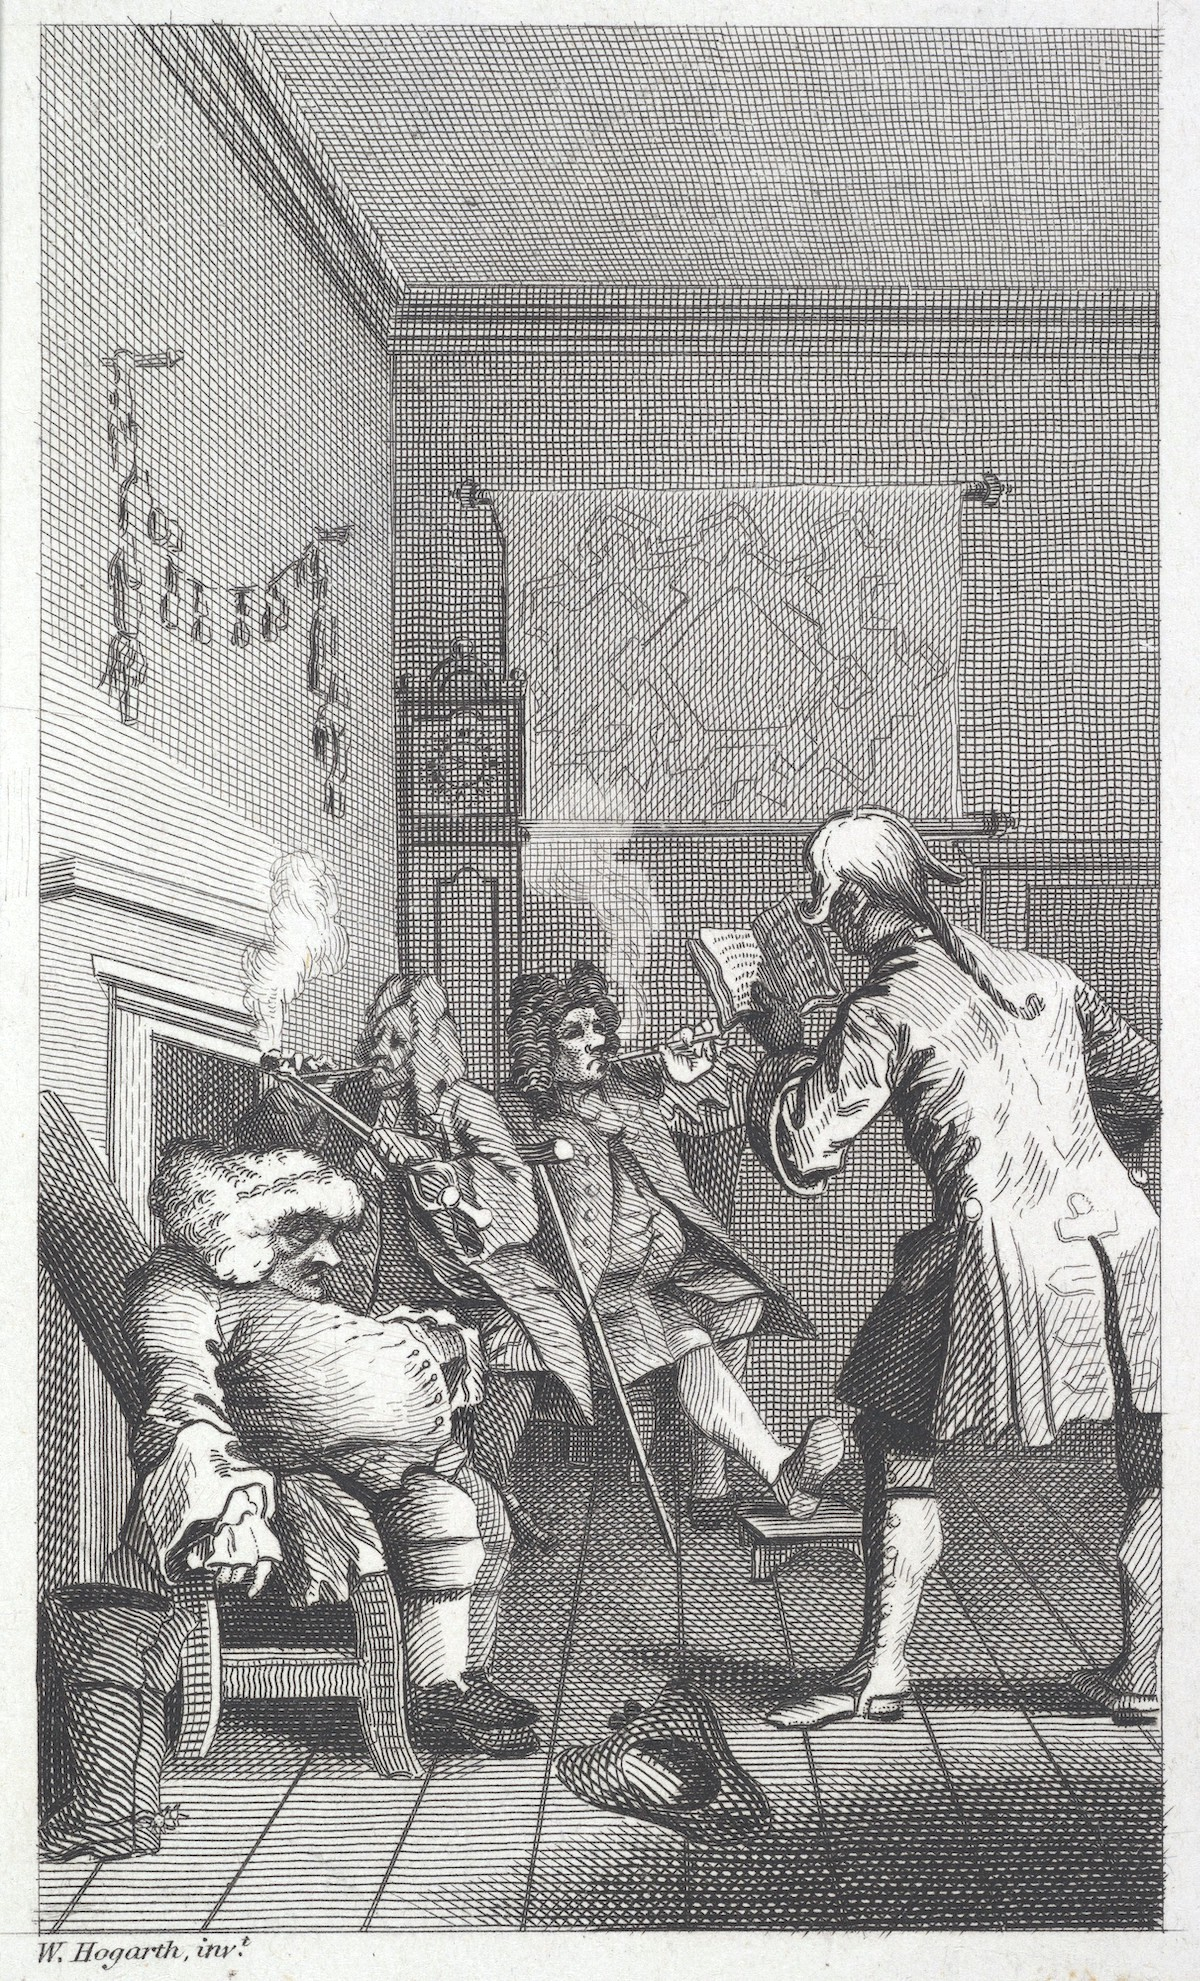
\includegraphics[width=166pt]{hogarth-front-1}
\newpage
\vbox{\openup 10pt\halign{\hss #\hss\cr
\hbox to 3em{T H E}\cr
\lower 2pt\hbox to 9em{\Large L I F E}\cr
\hbox to 3em{A N D}\cr
\lower 3pt\hbox to 15em{\Large O P I N I O N S}\cr
\textsc{o f}\cr
\hbox{\large\lsss{TRISTRAM SHANDY},}\cr
\lower-2pt\hbox{\textsc{\lss{Gentleman}.}}\cr
}}
\vfill
\vbox{\openup -2pt\halign to 180pt{\footnotesize #\cr
\quad Ταράσσει τοὺς Ἀνθρὠπους οὐ τὰ Πράγματα,\cr
ἀλλὰ τὰ περὶ τῶν Πραγμἀτων, Δογμἀτα.\hfill\cr}}
\vfill
\centerline{\lsss{VOL}.\quad I.}
\smallskip
\centerline{\textsc{The Second Edition}.}
\vfill
\centerline{\itshape\lsss{LONDON}:}
\centerline{\smaller Printed for R.\@ and J.\@ \lss{\textsc{Dodsley}} in \textit{Pall-Mall}.}
\centerline{M.DCC.LX.}

\newpage
\null
\newpage
\pagestyle{dedication}
\thispagestyle{empty}
\centerline{\small To the Right Honourable}
\vfill
\stick{\huge\  Mr. P I T T.\ }

\vfill

\bgroup
\fontsize{11}{15}\selectfont

\indent S I R,

\lettrine{N}{\,\ls{ever}} poor Wight of a De-\break
dicator had less hopes from\break
his Dedication, than I have from\break
this of mine ; for it is written in\break
a bye corner of the kingdom, and\break
in a retired thatch'd house, where\break
I live in a constant endeavour to\break
fence against the infirmities of ill\break
health, and other evils of life, by\catch{mirth;}
mirth; being firmly perfuaded that
every time a man smiles,\tsk but\break
more more so, when he laughs,\break
that it adds something to this Frag-\break
ment of Life.

I humbly beg, Sir, that you\break
will honour this book by taking\break
it \tsh (not under your Protection,\break
\tsh it must protect itself, but)\tsk\break
into the country with you; where,\break
if I am ever told, it has made\break
you smile, or can conceive it has\break
beguiled you of one moment's\break
pain\tsh I shall think myself as\break
happy as a minister of state;\tsh\break
perhaps much happier than any\catch{one}
one (one only excepted) that I have\break
ever read or heard of.

\bigskip

\rightline{\vbox{\openup 12pt\halign{\itshape #\cr\cr
\hfill I am, great Sir,\hfill\cr
\hfill (and what is more to your Honour,)\cr
\kern 62pt I am, good Sir,\hfill\cr
\kern 70pt Your Well-wisher,\hfill\cr
\hfill and most humble Fellow-Subject,\cr
\hfill\normalshape\textsc{The Author}.\cr}}}
\egroup

\newpage\null
\thispagestyle{empty}
\newpage
\setcounter{page}{1}
\pagestyle{folio}
\thispagestyle{empty}
\[\vbox{\openup 6pt\halign{\hss # \hss\cr
\addfontfeature{LetterSpace=12.0}\textsc{the}\cr
\addfontfeature{LetterSpace=12.0}LIFE and OPINIONS\cr
\addfontfeature{LetterSpace=12.0}\textsc{of}\cr
{\addfontfeature{LetterSpace=16.0}TRISTRAM SHANDY}, Gent.\cr}}\]

\vskip 6pt
\hrule
\setlength{\baselineskip}{14pt}  % 21*14 = 294+14 = 308 (for the catch)

\section{\lsss{CHAP}.\enspace I.}

\lettrine{I}{\,\ls{wish}} either my father or my mother,
or indeed both of them, as
they\break were in duty both equally bound to it, had minded what they were about
when they begot me; had they duly consider’d 
\stick{how much depended upon what they}
were then doing;\tsk  that not only the production of a rational Being
was concern’d in it, but that possibly the happy formation and temperature of
his body,\catch{per-} 
perhaps his genius and the very cast of\break
his mind;\tsk  and, for aught they knew to the contrary, even the fortunes of his
whole house might take their turn from 
\stick{the humours and dispositions which were}
\stick{then uppermost;\tsk  Had they duly}
\stick{weighed and considered all this, and}
\stick{proceeded accordingly,\tsk  I am verily}
\stick{persuaded I should have made a quite}
\stick{different figure in the world, from that,}
\stick{in which the reader is likely to see me.\tsk}
\stick{Believe me, good folks, this is not so}
\stick{inconsiderable a thing as many of you}
\stick{may think it;\tsk you have all, I dare say,}
\stick{\tight{heard of the animal spirits, as how they are}}
\stick{transfused from father to son, \&c.\,\&c.\tsk}
\stick{and a great deal to that purpose:\tsk  Well,}
\stick{you may take my word, that nine parts}
\stick{in ten of a man’s sense or his nonsense,}
\stick{his successes and miscarriages in this}
world depend upon their motions and ac-\catch{tivity,}
tivity, and the different tracks and trains you put them into, so that when they are
once set a-going, whether right or wrong, ’tis not a halfpenny matter,\tsk away
they go cluttering like hey-go mad; and by treading the same steps over and over
again, they presently make a road of it, as plain and as smooth as a garden-walk,
which, when they are once used to, the Devil himself sometimes shall not be able to
drive them off it.

\noindent
\stick{\indent \textit{Pray my dear}, quoth my mother, \textit{have}}
\stick{\textit{you not forgot to wind up the clock?}\tsk}
\textit{Good G\tsk!} cried my father, making
an exclamation, but taking care to moderate his voice at the same
time,\tsh \textit{Did ever woman, since the creation of the
world, interrupt a man with such a silly question?} Pray, what
was your father saying?\tsh\break 
Nothing.\patch{\ls{CHAP}.}

\section{\lsss{CHAP}.\enspace II.}

\quad \tsk Then, positively, there is nothing in the question that I can see, either good
\stick{or bad.\tsk  Then, let me tell you, Sir,}
it was a very unseasonable question at
least,\tsk  because it scattered and dispersed the animal spirits, whose business it
was to have escorted and gone hand-in-hand 
\stick{with the \ls{\textit{HOMUNCULUS}}, and con-}
ducted him safe to the place destined for his reception.

The \textsc{Homunculus}, Sir, in how-ever low and ludicrous a light he may appear,
in this age of levity, to the eye of folly or prejudice;\tsk  to the eye of reason
in scientifick research, he stands confess’d\tsk\break a \textsc{Being} guarded and
circumscribed with rights:\tsh  The minutest philosophers,\catch{who,} 
who, by the bye, have the most enlarged understandings, (their souls being in-\break 
versely as their enquiries) shew us incontestably, That the \textsc{Homunculus} is
created by the same hand,\tsk engender’d in the same course of nature,\tsk  endowed
with the same loco-motive powers and faculties with us:\tsk  That he consists,\break
as we do, of skin, hair, fat, flesh, veins,\break
\stick{arteries, ligaments, nerves, cartilages,}\break
bones, marrow, brains, glands, genitals, humours, and articulations;\tsk  is a Being
of as much activity,\tsk  and in all senses of the word, as much and as truly our
fellow-creature as my Lord Chancel-\break
\stick{lor of England.\tsk  He may be benefitted,}
he may be injured,\tsk  he may obtain redress;\tsk in a word, he has all the claims
\stick{and rights of humanity, which \textit{Tully},}
\textit{Puffendorf}, or the best ethick writers\catch{allow} allow to arise out of that state and relation.

Now, dear Sir, what if any accident had befallen him in his way
alone!\tsk\break  or that, through terror of it, natural to so young a
traveller, my little gentleman had got to his journey’s end
miserably 
\stick{spent;\tsk  his muscular strength and}
\stick{virility worn down to a thread;\tsk his}
\stick{own animal spirits ruffled beyond de-}
scription,\tsk  and that in this sad disorder’d state of
nerves, he had lain down a prey to sudden starts, or a series of
melancholy dreams and fancies for nine long, long months
together.\tsh  I tremble to think what a foundation had been laid
for a thousand weaknesses both of body and mind, which no skill of
the physician or the philosopher could ever afterwards have set
thoroughly to rights.\hfill
\catch{\ls{CHAP}.}

\section{\lsss{CHAP}.\enspace III.}

\lettrine{T}{\,o} my uncle Mr.\@ \textit{Toby Shandy} do~I\break
stand indebted for the preceding\break
\stick{anecdote, to whom my father, who was}
\stick{an excellent natural philosopher, and}
\stick{much given to close reasoning upon the}
\stick{smallest matters, had oft, and heavily,}
\stick{complain’d of the injury; but once more}
\stick{particularly, as my uncle \textit{Toby} well re-}
\stick{member’d, upon his observing a most}
\stick{unaccountable obliquity, (as he call’d it)}\break
in my manner of
setting up my top, and justifying the principles upon which I had
done it,\tsk  the old gentleman shook his head, and in a tone more
expressive by half of sorrow than reproach,\tsk  he said his heart
all along foreboded, and he saw it verified in this, and from a
thousand other observations he had made up-\catch{on} on me, That I should
neither think nor act like any other man’s
child:\tsk  \textit{But alas!} continued he, shaking his head a
second time, and wiping away a tear which was trickling down his
cheeks, \textit{My Tristram’s misfortunes began nine months before
ever he came into the world.}

\tsh My mother, who was sitting by,\break
\stick{look’d up,\tsk but she knew no more than}
\stick{her backside what my father meant,\tsk  but}
\stick{my uncle, Mr.\@ \textit{Toby Shandy}, who had}
\stick{been often informed of the affair,\tsk  un-}
derstood him very well.

\section{\lsss{CHAP}.\enspace IV.}

\lettrine{I}{ know} there are readers in the
world, as well as many other good people in it, who are no readers
at all,\tsk  who\catch{find} find themselves ill at ease, unless they are let
into the whole secret from first to last, of every thing which
concerns you.

It is in pure compliance with this humour of theirs, and from a
backwardness in my nature to disappoint any one soul living, that I
have been so very particular already. As my life and opinions are
likely to make some noise in the world, and, if I conjecture right,
will take in all ranks, professions, and denominations of men
whatever,\tsk  be no less read than the \textit{Pilgrim’s
Progress} itself\tsk  and in the end, prove the very thing
which \textit{Montaigne} dreaded his essays should turn out, that is,
a book for a parlour-window;\tsk  I find it necessary to consult
every one a little in his turn; and therefore must beg pardon for going on a little farther in the same way:
For which cause, right glad\catch{I} I am, that I have begun the history of
myself in the way I have done; and that I am able to go on, tracing
every thing in it, as \textit{Horace} says, \textit{ab Ovo.}

\textit{Horace}, I know, does not recommend this fashion
altogether: But that gentleman is speaking only of an epic poem or
a tragedy;\tsk  (I forget which)\tsk besides, if it was not so, I
should beg Mr.\@ \textit{Horace’s} pardon;\tsk  for in writing
what I have set about, I shall confine myself neither to his rules,
nor to any man’s rules that ever lived.

To such however as do not choose to 
go so far back into these things, I can\break
give no better advice than that they\break
skip over the remaining part of this\break 
Chapter; for I declare before hand, ’tis\catch{wrote}
wrote only for the curious and inquisitive.

\noindent
\stick{\indent
\leaders\hrule width 1pt height 3.14pt depth -2.6pt\hfill
\hbox{Shut the door.}
\leaders\hrule width 1pt height 3.14pt depth -2.6pt\hfill}\break
I was begot in the night betwixt the first \textit{Sunday} and the first
\textit{Monday} in the month of \textit{March}, in the year of our Lord one thousand
seven hundred and eighteen.\break
I am positive I was.\tsk  But how I came to be so very
particular in my account of a thing which happened before I was born, is owing to
another small anecdote known only in our own family, but now made publick for the
better clearing up this point.

My father, you must know, who was originally a \textit{Turkey}
merchant, but had left off business for some years, in order to
retire to, and die upon, his paternal estate in the county of\tsh, 
was, I believe,\catch{one} one of the most regular men in
every thing he did, whether ’twas matter of business, or
matter of amusement, that ever lived. As a small specimen of this
extreme exactness of his, to which he was in truth a slave,\tsk he had
made it a rule for many years of his life,\tsk  on the first
\textit{Sunday night} of every month throughout the whole
year,\tsk  as certain as ever the \textit{Sunday night}
came,\tsk  to wind up a large house-clock, which we had standing
on the back-stairs head, with his own hands:\tsk  And being
somewhere between fifty and sixty years of age at the time I
have been speaking of,\tsk  he had likewise gradually
brought some other little family concernments to the same period,
in order, as he would often say to my uncle \textit{Toby}, to get
them all out of the way at one time, and be no more plagued\catch{and}
and pestered with them the rest of the month.

It was attended but with one misfortune, which, in a great
measure, fell upon myself, and the effects of which I fear\break
\stick{I shall carry with me to my grave; na-}
mely, that, from an unhappy association
of ideas, which have no connection in nature, it so fell out at
length, that my poor mother could never hear the said clock wound
up,\tsk  but the thoughts of some other things unavoidably
popp’d into her head\tsk  \hbox{{\small\itshape\egb\&} \textit{vice
versâ:}}\tsk  which strange combination of ideas, the
sagacious \textit{Locke}, who certainly understood the nature of
these things better than most men, affirms to have produced\break more
wry actions than all other sources\break of prejudice whatsoever.\\
\indent But this by the bye.\hfill\catch{Now}

Now it appears by a memorandum in my father’s pocket-book, which now lies upon
the table, \lqq That on \textit{Lady-day}, which was on the 25th of
the same month 
\stick{in which I date my geniture,\tsk  my father}
set out upon his journey to \textit{London}, with my eldest brother
\textit{Bobby}, to fix him at\break\textit{Westminster} school;” and,
as it appears from the same authority, \lqq That he did not get
down to his wife and family till the \textit{second week} in
\textit{May} following,”\tsk  it brings the thing almost to a
certainty.\break
However, what follows in the beginning of the next
chapter, puts it beyond all possibility of a doubt.

\tsh  But pray, Sir, What was your father doing
all \textit{December},\tsk\textit{January}, and
\textit{February?}\tsh  Why, Madam,\tsk  he was\break all that
time afflicted with a Sciatica.
\hfill\catch{\ls{CHAP}.}

\section{\lsss{CHAP}.\enspace V.}

\lettrine{O}{\,n} the fifth day of \textit{November},
1718, which to the æra fixed on, was as\break 
\stick{\tight{near nine kalendar months as any husband}}
\stick{could in reason have expected,\tsk  was I}\break
\stick{\textit{Tristram Shandy}, Gentleman, brought}
\stick{forth into this scurvy and disasterous}
\stick{world of ours.\tsk  I wish I had been born}
in the Moon, or in any of the
planets, (except \textit{Jupiter} or \textit{Saturn}, because I never
could bear cold weather) for it could not well have fared worse
with me in any of them (though I will not answer for \textit{Venus})
than it has in this vile, dirty planet of ours,\tsk  which,
o’ my conscience, with reverence be it spoken, I take to be
made up of the shreds and clippings of the rest;\tsh  not
but the planet is well enough, provided a man could be born\catch{in} in it
to a great title or to a great estate; or could any how contrive to
be called up to public charges, and employments of dignity or
power;\tsh  but that is not my case;\tsh  and
therefore every man will speak of the fair as his own market has
gone in it;\tsk  for which cause I affirm it over
again to be one of the vilest worlds that ever was made;\tsk  for
I can truly say, that from the first hour I drew my breath in it,
to this, that I can now scarce, draw it at all, for an asthma I got
in scating against the wind in \textit{Flanders;}\tsk\break
I have been the continual sport of what the world calls fortune; and though I will
not wrong her by saying, She has ever made me feel the weight of any great or signal
evil;\tsk  yet with all the good temper in the world I affirm it of her, that in
every stage of my life, and at every turn and corner where she could\catch{get} get fairly
at me, the ungracious Duchess has pelted me with a set of as pitiful misadventures
and cross accidents as ever small \ls{\textsc{Hero}} sustained.

\section{\lsss{CHAP}.\enspace VI.}

\lettrine{I}{\,n} the beginning of the last chapter,
I inform’d you exactly \textit{when} I was born;\tsk but I did not inform
you \textit{how}.\break\textit{No}, that particular was reserved entirely 
\stick{for a chapter by itself;\tsk  besides, Sir, as}
you and I are in a manner
perfect stran\-gers to each other, it would not have been proper to
have let you into too many circumstances relating to myself all at
once.\tsk You must have a little patience. I have undertaken, you see, to write not only my life,
but my opinions also; hoping and expecting that your knowledge\catch{of}
of my character, and of what kind of a
mortal I am, by the one, would give you
\stick{a better relish for the other: As you}
proceed farther with me, the slight ac\-quaintance, which is now beginning betwixt us,
will grow into familiarity; and that unless one of us is in fault, will\break
terminate in friendship.\tsk  \textit{O diem
prae\-clarum!}\tsh  then nothing which has touched me will be
thought trifling in its nature, or tedious in its telling.\break
Therefore, my dear friend and companion, if you should think me
somewhat sparing of my narrative on my first setting out,\tsk  bear
with me,\tsk  and let me go on, and tell my story my own
way:\tsh  or, if I should seem now and then to trifle upon the
road,\tsk  or should sometimes put on a fool’s cap with a
bell to it, for a moment or two as we pass along,\tsk  don’t
fly off,\tsk  but rather courteously give me\catch{credit} credit for a little
more wisdom than appears upon my outside;\tsk  and as we jogg on, either laugh with
me, or at me, or in short, do any thing,\tsk  only keep your temper.

\section{\lsss{CHAP}.\enspace VII.}

\lettrine{I}{\,n} the same village where my father
and my mother dwelt, dwelt also a thin, upright, motherly, notable,
good\break old body of a midwife, who with the help of a little plain
good sense, and some years full employment in her business, in
which she had all along trusted little to her own efforts, and a
great deal to those of dame nature,\tsk  had acquired, in her way,
no small degree of reputation in the world:\tsk  by which word
\textit{world}, need I in this place inform your worship,\catch{that}
that I would be understood to mean no 
more of it, than a small circle described 
\stick{upon the circle of the great world, of}
\stick{four \textit{English} miles diameter, or there-}
abouts, of which the cottage where the good old woman lived is supposed to be
the centre.\tsh  She had been left, it seems, a widow in great distress, with three or
four small children, in her forty-seventh year; and as she was at that time a person
of decent carriage,\tsk  grave de-\break
\stick{portment,\tsk  a woman moreover of few}
words, and
withall an object of compassion, whose distress and silence under it call’d out the
louder for a friendly lift:\break the wife of the parson of the parish was touch’d with
pity; and having often la\-mented an inconvenience to which her husband’s flock had
for many years been exposed, inasmuch, as there was no such thing as a midwife, of
any kind or de-\catch{gree} gree to be got at, let the case have been never so urgent, within
less than six or seven long miles riding; which said seven long miles in dark nights
and dismal\break roads, the country thereabouts being no\-\stick{thing but a deep clay, was almost
equal to}\break\stick{\tight{fourteen; and that in effect was sometimes}} next to having no midwife at
all; it came\break
\stick{into her head, that it would be doing as} seasonable a kindness to the
whole parish, as to the poor creature herself, to get her a little instructed in
some of the plain\break
\stick{principles of the business, in order to set}
her up in it. As no
woman thereabouts was better qualified to execute the plan she had formed than
herself, the Gentle\-woman very charitably undertook it; and having great influence
over the female part of the parish, she found no difficulty in effecting it to the
utmost of her wishes. In truth, the parson join’d his interest\catch{with} with his wife’s in
the whole affair, and in order to do things as they should be,\break and give the poor
soul as good a title by law to practise, as his wife had given by institution,\tsk
he cheerfully paid the fees for the ordinaries licence himself, amounting, in the
whole, to the sum of eighteen shillings and fourpence; so that betwixt them both,
the good woman was fully invested in the real and corporal possession of her office,
together with all its \textit{rights, members, and appurtenances whatsoever.}

These last words, you must know,\break
\stick{were not according to the old form in} 
\stick{which such licences, faculties, and powers}
\stick{usually ran, which in like cases had here-}
\stick{tofore been granted to the sisterhood.} But
it was according to a neat \textit{Formula} of \textit{Didius} his own devising, who
having\catch{a} a particular turn for taking to pieces, and new framing over again all
kind of instruments in that way, not only hit upon this dainty amendment, but coaxed
many of the old licensed matrons in the neighbourhood, to open their faculties
afresh, in order to have this wham-wham of his inserted.

I own I never could envy \textit{Didius} in
\stick{these kinds of fancies of his:\tsk  But every}
\stick{man to his own taste.\tsk  Did not Dr.\,\textit{Ku-}}
\textit{nastrokius}, that great man, at his leisure hours, take the
greatest delight imagin\-able in combing of asses tails, and plucking
the dead hairs out with his teeth, though he had tweezers always in
his
\stick{pocket? Nay, if you come to that, Sir, have} not the wisest of
men in all ages, not excepting \textit{Solomon} himself,\tsk  have
they not had their
\textsc{Hobby-Horses};\tsk  their running\catch{horses,}
horses,\tsk  their coins and their cockle-shells, their drums and
their trumpets, their fiddles, their pallets,\tsk  their maggots
and their butterflies?\tsk  and so long as a man rides his
\textsc{Hobby-Horse} peaceably and quietly
along the King’s highway, and neither compels you or me to
get up behind him,\tsk  pray, Sir, what have either you or I to do
with it?

\section{\lsss{CHAP}.\enspace VIII.}

\quad\tsk \textit{De gustibus non est
disputandum;}\break\tsk  that is, there is no disputing against
\textsc{Hobby-Horses}; and for my part, I
seldom do; nor could I with any sort of grace, had I been an enemy
to them at the bottom; for happening, at certain intervals and
changes of the moon, to be both fiddler and painter, according as
the fly stings:\tsk  Be it known to you, that I\catch{keep}
\stick{keep a couple of pads myself, upon}
which, in their turns, (nor do I care who knows
it) I frequently ride out and take 
the air;\tsk  tho’ sometimes, to my shame\break
be it spoken, I take somewhat longer\break
journies than what a wise man would\break
think altogether right.\tsk  But the truth\break
is,\tsk  I am not a wise man;\tsk  and besides am a mortal of so little consequence in the world,
it is not much matter what I do: so I seldom fret or fume at all
about it: Nor does it much disturb my rest, when I see such great
Lords and tall Personages as hereafter follow;\tsk  such, for
instance, as my Lord A, B, C, D, E, F, G, H, I, K, L, M, N, O, P,
Q, and so on, all of a row, mounted upon their several
horses;\tsk  some with large stirrups, getting on in a more grave
and sober pace;\tsh  others on the contrary, tuck’d up to
their very chins, with whips across\catch{their} their mouths, scouring and
scampering it away like so many little party-colour’d devils
astride a mortgage,\tsh  and as if\break
some of them were resolved to break\break
their necks.\tsh  So much the better\tsk  say\break
I~to myself;\tsk  for in case the worst should happen, the world will
make a shift to do excellently well without them; and for the
rest,\tsh  why\tsh  God speed
them,\tsk  e’en let them ride on without opposition
from me; for were their lordships unhorsed this very
night\tsk  ’tis\break ten to one but that many of them would
be worse mounted by one half before tomorrow
morning.

Not one of these instances therefore can be said to break in upon my rest.\tsk\break
But there is an instance, which I own puts me off my guard, and that is, when I see
one born for great actions, and what is\catch{still} still more for his honour,
whose nature ever inclines him to good ones;\tsh\break  when I behold such a one, my
Lord, like yourself, whose principles and conduct are as generous and noble as his
blood, and whom, for that reason, a corrupt world cannot spare one moment;\tsk  when
\stick{I see such a one, my Lord, mounted,} though it is but for a minute beyond the
time which my love to my country has prescribed to him, and my zeal for his glory
wishes,\tsk  then, my Lord, I cease to be a philosopher, and in the first transport
of an honest impatience, I wish the \textsc{Hobby-Horse}, with all his fraternity,
at the Devil.

My Lord,\\[-24pt]
\lettrine{\rlap{\normalsize “}\lower-12pt\hbox{\normalsize \lqq }I}{ \ls{maintain}} this to
be a dedication,\break
notwithstanding its singularity in\break
\stick{\lqq  the three great essentials of matter,}\catch{\lqq form,}
\stick{\lqq  form, and place: I beg, therefore, you}
\stick{\lqq  will accept it as such, and that you will}
\stick{\lqq  permit me to lay it, with the most re-}
\stick{\lqq  spectful humility, at your Lordship’s}
\stick{\lqq  feet\tsk  when you are upon them,\tsk}
\stick{\lqq  which you can be when you please;\tsk}
\stick{\lqq  and that is, my Lord, when ever there}
\stick{\lqq  is occasion for it, and I will add, to the}
\stick{\lqq  best purposes too. I have the honour}
\stick{\lqq  to be,\hfill}

\noindent\rightline{\vbox{\openup8pt\halign{\hss#\cr
\textit{My Lord},                       \kern 60pt\cr
\textit{Your Lordship’s most obedient}, \kern 24pt\cr
\textit{and most devoted},              \kern 50pt\cr
\textit{and most humble servant},       \kern  6pt\cr
\ls{\textsc{Tristram Shandy}}.\cr
}}}
\vskip 36pt
\rightline{\ls{CHAP}.}
\newpage
\section{\lsss{CHAP}.\enspace IX.}

\lettrine{I}{ solemnly} declare to all mankind,
that the above dedication was made for no one Prince, Prelate,
Pope, or Potentate,\tsk  Duke, Marquis, Earl, Viscount, or Baron, of this, or any other Realm in
Christendom;\tsh  nor has it yet been hawk’d about, or
offered publickly or privately, directly or indirectly, to any one
person or personage, great or small; but is honestly a true
Virgin-Dedication\break untried on, upon any soul living.

I labour this point so particularly,\break merely to remove any
offence or objection which might arise against it from the manner
in which I propose to make the most of it;\tsk  which is the
putting\catch{it} it up fairly to public sale; which I now do.

\tsh  Every author has a way of his
own, in bringing his points to bear;\tsk  for
my own part, as I hate chaffering and
higgling for a few guineas in a dark\break
entry;\tsk  I resolved within myself, from
the very beginning, to deal squarely and 
openly with your Great Folks in this affair, 
and try whether I should not come
off the better by it.

If therefore there is any one Duke, 
\stick{Marquis, Earl, Viscount, or Baron, in}
\stick{these his Majesty’s dominions, who stands}
\stick{in need of a tight, genteel dedication,}
\stick{and whom the above will suit, (for by}
\stick{the bye, unless it suits in some degree, I}
\stick{will not part with it)\tsh  it is much at}
his service for fifty guineas;\tsh  which\catch{I}
I am positive is twenty guineas less
than it ought to be afforded for, by any man of genius.

My Lord, if you examine it over\break 
again, it is far from being a gross piece\break
of daubing, as some dedications are.\break
The design, your
Lordship sees, is good, 
\stick{the colouring transparent,\tsk  the
drawing}
not amiss;\tsk  or to speak more like a man of
science,\tsk  and measure my piece in the painter’s scale,
divided into 20,\tsk  I~believe, my Lord, the out-lines will turn
out as 12,\tsk  the composition as 9,\tsk  the colouring as
6,\tsk  the expression 13 and a half,\tsk  and the
design,\tsk  if I may be allowed, my Lord, to understand my own
\textit{design}, and supposing absolute perfection in designing, to
be as 20,\tsk  I think it cannot well fall short of 19. Besides
all this,\tsk  there is keeping in it, and\catch{the} the dark strokes in the
\textsc{Hobby-Horse}, (which is a secondary
figure, and a kind of back-ground to the whole) give great force to the
principal lights in your own figure, and make it come off
wonderfully;\tsk  and besides, there is an air of originality in
the \textit{tout ensemble.}

Be pleased, my good Lord, to order the sum to be paid into the
hands of Mr.\break\textit{Dodsley}, for the benefit of the author; and in
the next edition care shall be ta-\break ken that this chapter be expunged,
and your Lordship’s titles, distinctions, arms, and good
actions, be placed at the front of the preceding chapter: All
which, from the words, \textit{De gustibus non est disputandum}, and
whatever else in this book relates to
\ls{\textsc{Hobby-Horses}}, but no more, shall
stand dedicated to your Lordship.\tsk\break  The rest I dedicate to the
\textsc{Moon}, who, by\catch{the} the bye, of all the \textsc{Patrons} or
\textsc{Matrons} I can think of, has most power to set my
book a-going, and make the world run mad after it.

\vskip-6pt

\textit{Bright Goddess},

\vskip-6pt

If thou art not too busy with \textsc{Candid} and Miss
\textsc{Cunegund’s} affairs,\tsk  take \textit{Tristram
Shandy}’s under thy protection also.

\vskip-6pt

\enlargethispage\baselineskip

\section{\lsss{CHAP}.\enspace X.}

\lettrine{W\,}{hatever} degree of small merit, the
act of benignity in favour of the midwife might justly claim, or in
whom that claim truly rested,\tsk  at first sight seems not very
material to this\break history;\tsh  certain however it was, that
the gentlewoman, the parson’s wife, did run away at that time
with the whole of it: And yet, for my life, I cannot help thinking
but that the parson himself,\catch{tho’} tho’ he had not the good fortune to
hit upon the design first,\tsk  yet, as he heartily concurred in
it the moment it was laid before him, and as heartily parted with\break
his money to carry it into execution,\break had a claim to some share of
it,\tsk  if not to a full half of whatever honour was due to
it.

The world at that time was pleased to determine the matter
otherwise.

Lay down the book, and I will allow you half a day to give a
probable guess at the grounds of this procedure.

Be it known then, that, for about five years before the date of
the midwife’s licence, of which you have had so
circumstantial an account,\tsk  the parson we have to do with, had
made himself a\catch{country-} country-talk by a breach of all decorum, which he
had committed against himself, his station, and his
office;\tsk  and that was in never appearing better, or otherwise
mounted, than upon a lean, sorry,\break
\stick{jack-ass of a horse, value about one}
pound fifteen shillings; who, to shorten all description of
him, was full brother to\break \textit{Rosinante}, as far as similitude
congenial could make him; for he answered his description to a
hair-breadth in every\break
\stick{thing,\tsk  except that I do not remember}
’tis any where said, that \textit{Rosinante} was broken-winded;
and that, moreover, \textit{Rosinante}, as is the happiness of most
\textit{Spanish} horses, fat or lean,\tsk  was undoubtedly a horse
at all points.

I know very well that the \ls{\textsc{Hero}}’s\break
horse was a horse of chaste deportment, which may
have given grounds for a\catch{con-} 
\stick{contrary opinion: But it is as certain at}
the same time that \textit{Rosinante’}s continen\-cy (as may
be demonstrated from the adventure of the \textit{Yanguesian}
carriers) proceeded from no bodily defect or cause whatsoever, but
from the temperance and orderly current of his blood.\tsk  And\break
let me tell you, Madam, there is a great deal of very good chastity in the world, in
behalf of which you could not say more for your life.

Let that be as it may, as my purpose is to do exact justice to
every creature brought upon the stage of this dramatic
work,\tsk  I could not stifle this distinction in favour of Don
\textit{Quixote’}s horse;\tsh  in all other points, the
parson’s horse, I say, was just such another,\tsk for he was as
lean, and as lank, and as sorry a jade, as \ls{\textsc{Humility}}
herself could have bestrided.\catch{In}

In the estimation of here and there a man of weak judgment, it was greatly
in the parson’s power to have helped the figure of
this horse of his,\tsk  for he was master of a very handsome
demi-peak’d saddle, quilted on the seat with green plush,
garnished with a double row of silver-headed studs, and a noble
pair of shining brass stirrups, with a housing altogether
suitable, of grey superfine cloth, with an edging of black lace,
terminating in a deep, black, silk fringe, \textit{poudrè
d’or},\tsk  all which he had purchased in the pride and prime of
his life, together with a grand embossed bridle, ornamented at
all points as it should be.\tsh  But not caring to banter his
beast, he had hung all these up behind his study door;\tsk and, in
lieu of them, had seriously befitted\break him with just such a bridle
and such\catch{a} a saddle, as the figure and value of such a steed might
well and truly deserve.

In the several sallies about his parish, 
and in the neighbouring visits to the\break
gentry who lived around him,\tsh  you\break will easily
comprehend, that the parson, so appointed, would both hear and see
enough to keep his philosophy from\break
rusting. To speak the truth, he never
could enter a village, but he caught the attention
of both old and young.\tsh  La-\break
\stick{bour stood still as he pass’d\tsh  the bucket}
\stick{hung suspended in the middle of the}
\stick{well,\tsk  the spinning-wheel forgot its}
\stick{round,\tsh  even chuck-farthing and}\break shuffle-cap themselves
stood gaping till he had got out of sight; and as his\break
movement was
not of the quickest, he had generally time enough upon his\break
hands to make his observations,\tsk  to hear\catch{the} the groans of the
serious,\tsh and the laughter of the light-hearted;\tsk all which he
bore with excellent tranquillity.\tsk  His character was,\tsk  he
loved a jest in his heart\tsk  and as he saw himself in the true
point of ridicule, he would say he could not be angry with others
for seeing him in a light, in which he so strongly saw himself: So
that to his friends, who knew his foible was not the love of money,
and who therefore made the less scruple in bantering the
extravagance of his humour,\tsk  instead of giving the true
cause,\tsk  he chose rather to join in the laugh against himself;
and as he never carried one single ounce of flesh upon his own bones, being altogether
as spare a figure as his beast,\tsk  he would sometimes insist
upon it, that the horse was as good as the rider
deserved;\tsk  that they were, centaur-like,\tsk  both of a
piece. At other\catch{times,} times, and in other moods, when his spirits were
above the temptation of false wit,\tsk  he would say, he found
himself going off fast in a consumption; and, with great gravity,
would pretend, he could not bear the sight of a fat horse, without
a dejection of heart, and a sensible alteration in his pulse; and
that he had made choice of the lean one he rode upon, not only to
keep himself in countenance, but in spirits.

At different times he would give fifty humorous and apposite
reasons for riding a meek-spirited jade of a broken-\break 
winded horse,
preferably to one of mettle;\tsk  for on such a one he could sit
mechanically, and meditate as delightfully \textit{de vanitate mundi et
fugâ sæculi}, as with the advantage of a
death’s head before him;\tsk  that, in all other
exercitations, he\catch{could}
could spend his time, as he rode slowly along,\tsk  to as
much account as in his study;\tsk  that he could draw up an
argument in his sermon,\tsk  or a hole in his breeches, as
steadily on the one as in the other;\tsk  that brisk trotting and
slow argumentation, like wit and judgment, were two incompatible
movements.\tsk  But that upon his steed\tsk  he could unite and
reconcile every thing,\tsk  he could compose his sermon,\tsk  he
could compose his cough,\tsh  and, in case nature gave a
call that way, he could likewise compose himself to sleep.\tsk  In
short, the parson upon such encounters would assign any cause, but
the true cause,\tsk  and he with\-held the true one, only out of a
nicety of temper, because he thought it did honour to him.\patch{But}

But the truth of the story was as follows: In the first years of
this gentleman’s life, and about the time when the superb saddle
and bridle were purchased by him, it had been his manner, or
vanity, or call it what you will,\tsk  to run into the opposite
extream.\tsk  In the language of the county where he dwelt, he
was said to have loved a good horse, and generally had one of
the best in the whole parish standing in his stable always ready
\stick{for saddling: and as the nearest midwife,}\break
as I told you, did not
live nearer to the village than seven miles, and in a vile
country,\tsh  it so fell out that the poor\break gentleman was scarce
a whole week together without some piteous application for his
beast; and as he was not an un\-kind-hearted man, and every case
was more pressing and more distressful than the last,\tsk  as
much as he loved his beast,\catch{he} he had never a heart to refuse
him; the upshot of which was generally this, that his horse was
either clapp’d, or spavin’d, or greaz’d;\tsk  or he was
twitter-bon’d, or broken-winded, or something, in short, or
other had befallen him, which would let him carry no flesh;\tsk
so that he had every nine or ten months a bad horse to get rid
of,\tsk  and a good horse to purchase in his stead.

What the loss in such a balance might amount to, \textit{communibus
annis}, I would leave to a special jury of sufferers in the same traffick,
to determine;\tsk  but let it be what it would, the honest
gentleman bore it for many years without a murmur, till at length,
by repeated ill accidents of the kind, he found it necessary to
take the thing under consideration; and upon weighing the whole,
and summing it up\catch{in} in his mind, he found it not only disproportioned
to his other expences, but withal so heavy an article in itself, as
to disable him from any other act of generosity in his parish:
Besides this, he considered that with half the sum thus galloped
away, he could do ten times as much good;\tsk  and what still
weighed more with him than all other considerations put together,
was this, that it confined all his charity into one particular
channel, and where, as he fancied, it was the least wanted, namely,
to the child-bearing and child-getting part of his\break parish;
reserving nothing for the impotent,\tsk  nothing for the
aged,\tsk  nothing for the many comfortless scenes he was 
\stick{hourly called forth to visit, where po-}
\stick{verty, and sickness, and affliction dwelt}\break together.\patch{For}

For these reasons he resolved to discontinue the expence; and
there appeared but two possible ways to extricate him clearly out
of it;\tsk  and these were, either to make it an irrevocable law
never more to lend his steed upon any application
whatever,\tsk  or else be content to ride the last poor devil,
such as they had made him, with all his aches and infirmities, to
the very end of the chapter.

As he dreaded his own constancy in the first,\tsk  he very
chearfully betook himself to the second; and tho’ he could very
well have explain’d it, as I said, to his honour,\tsk  yet, for
that very reason, he had a spirit above it; choosing rather to bear
the contempt of his enemies, and the laughter of his friends, than
undergo the pain of telling a story, which might seem a panegyric
upon himself.\patch{I}

I have the highest idea of the spiritual and refined sentiments of this reverend
gentleman, from this single stroke in his character, which I think comes up to any
of the honest refinements of the peerless knight of \textit{La Mancha}, whom, by the
bye, with all his follies, I love more, and would actually have gone farther to have
paid a visit to, than the greatest hero of antiquity.

But this is not the moral of my story: The thing I had in view
was to shew the temper of the world in the whole of this
affair.\tsk  For you must know, that so long as this explanation
would have done the parson credit,\tsk  the devil a soul could
find it out,\tsk  I suppose his enemies would not, and that his
friends could not.\tsh  But no sooner did he bestir himself in
behalf of the midwife, and pay the expences of\catch{the} the ordinary’s
licence to set her up,\tsk  but the whole secret came out; every
horse he had lost, and two horses more than ever he had lost,
with all the circumstances of their destruction, were known and
distinctly remembered.\tsk  The story ran like wild-fire.\tsk\lqq The parson
had\break
\lqq a returning fit of pride which had just\break
\lqq seized him; and he was going to be\break
\lqq well mounted once again in his life;\break
\lqq and if it was so, ’twas plain as the sun\break
\lqq at noon-day, he would pocket the ex-\break
\lqq pence of the licence ten times told the\break
\lqq very first year:\tsk  so that every body\break
\lqq was left to judge what were his views\break
\lqq in this act of charity.”

What were his views in this, and in every other action of his
life,\tsk  or rather what were the opinions which floated in the
brains of other people concerning it,\catch{was} was a thought which too much
floated in his own, and too often broke in upon his rest, when he
should have been sound asleep.

About ten years ago this gentleman had the good fortune to be
made entirely easy upon that score,\tsk  it being just so long
since he left his parish,\tsk  and the whole world at the same
time behind him,\tsk  and stands accountable to a judge of whom he
will have no cause to complain.

But there is a fatality attends the actions of some men: Order
them as they will, they pass thro’ a certain medium, which so twists and refracts them from their true
directions\tsh  that, with all the titles to praise which a
rectitude of heart can give, the doers of them are\catch{ne-} nevertheless
forced to live and die without it.

Of the truth of which, this gentleman was a painful
example.\tsh  But to know by what means this came to
pass,\tsk  and to make that knowledge of use to you, I~insist upon
it that you read the two following chapters, which contain such a
sketch of his life and conversation, as will carry its moral along
with it.\tsk  When this is done, if nothing stops us in our way,
we will go on with the midwife.

\section{\lsss{CHAP}.\enspace XI.}

\lettrine{Y}{\,\ls{orick}} was this parson’s name, and, what is very remarkable in it, (as
appears from a most antient account of the family, wrote upon strong vellum,\catch{and} and
now in perfect preservation) it had been exactly so spelt for near,\tsk  I was
within an ace of saying nine hundred\break
\stick{years;\tsh  but I would not shake my}
\stick{credit in telling an improbable truth,}
\stick{however indisputable in itself;\tsh  and}
therefore I
shall content myself with only saying,\tsh  It had been exactly so spelt, without the
least variation or transposition of a single letter, for I do not know how long;
which is more than I would venture to say of one half of the best sur-\break 
names in the
kingdom; which, in a course of years, have generally undergone as many chops and
changes as their owners.\tsk  Has this been owing to the pride, or to the shame of
the respective proprietors?\tsk  In honest truth, I think sometimes to the one, and
sometimes to the other, just as the temptation has wrought. But a villainous affair
it is, and will one\catch{day} day so blend and confound us all together,
\stick{that no one shall be able to stand up and}
swear, \lqq That his own great grand fa-\break
\lqq ther was the man who did either this\break
\lqq or that.\,” 

\vspace\parskip
This evil had been sufficiently fenced 
\stick{against by the prudent care of the \textit{Yorick}’s}
family, and their religious
preservation of these records I quote, which do further inform us,
That the family was originally of \textit{Danish} extraction, and had
been transplanted into England as early as in the reign of
\textit{Horwendillus}, king of \textit{Denmark}, in whose court it
seems, an ancestor of this Mr.\@ \textit{Yorick}’s, and from whom
he was lineally descended, held a considerable post to the day of
his death. Of what nature this considerable post was, this record
saith not;\tsk  it only adds, That, for near two centuries, it had
been totally\catch{abo-} abolished, as altogether unnecessary, not only in that
court, but in every other court of the Christian world.

It has often come into my head, that 
\stick{this post could be no other than that of}
the king’s chief Jester;\tsk  and that
\textit{Hamlet}’s \textit{Yorick}, in our \textit{Shakespear},
many of whose plays, you know, are founded upon authenticated
facts,\tsk was certainly the very man.

I have not the time to look into \textit{Saxo-Grammaticus}’s
\textit{Danish} history, to know the certainty of this;\tsk  but if
you have leisure, and can easily get at the book, you may do
it full as well yourself.

I had just time, in my travels through \textit{Denmark} with Mr.\@
\textit{Noddy}’s eldest son, whom, in the year 1741, I
accompanied\catch{as} as governor, riding along with him at a
\stick{prodigious rate thro’ most parts of \textit{Europe},}
and of which original journey
perform’d by us two, a most delectable narrative will be given in
the progress of this work.\break
I had just time, I say, and that was
all, to prove the truth of an observation made by a long sojourner
in that country;\tsh\break namely, “That nature was
neither very lavish, nor was she very stingy in her\break
\stick{gifts of genius and capacity to its inha-}
\stick{bitants;\tsk  but, like a discreet parent, was}
moderately kind to them all; observing such an equal tenor in
the distribution of her favours, as to bring them, in those points,
pretty near to a level with each other; so that you will meet with
few instances in that kingdom of refin’d parts; but a great
deal of good plain hous\-hold understanding amongst all
ranks of\catch{people,}
\stick{people, of which every body has a share;”}
which is, I think, very right.

With us, you see, the case is quite different:\tsk  we are all
ups and downs in this matter;\tsk  you are a great
genius;\tsk\break  or ’tis fifty to one, Sir, you are a great
\stick{dunce and a blockhead;\tsk  not that there}
\stick{is a total want of intermediate steps,\tsk}
\stick{no,\tsk  we are not so irregular as that comes}
to;\tsk  but the two extremes are more common, and in a
greater degree in this unsettled island, where nature, in her gifts
and dispositions of this kind, is most whimsical and capricious;
fortune herself not being more so in the bequest of her goods and
chattels than she.

This is all that ever stagger’d my faith in regard to
\textit{Yorick}’s extraction, who, by what I can remember of
him, and by all\catch{the} 
the accounts I could ever get of him,\break
seemed not to have had one single drop\break
of \textit{Danish} blood in his whole crasis; in\break
\stick{nine hundred years, it might possibly have}
\stick{all run out:\tsh  I will not philosophize}
\stick{one moment with you about it; for hap-}
\stick{pen how it would, the fact was this:\tsk}  
\stick{That instead of that cold phlegm and}
\stick{exact regularity of sense and humours, you}
\stick{would have look’d for, in one so extract-}
ed;\tsk  he was, on the contrary, as mercurial and
sublimated a composition,\tsk\break
as heteroclite a creature in all
his declensions;\tsk  with as much life and whim, and
\textit{gaité de cœur} about him, as the kindliest
climate could have engendered and put together. With all this sail,
poor \textit{Yorick} carried not one ounce of ballast; he was utterly
unpractised in the world; and at the age of twenty-six, knew just
about as well how to steer his course\catch{in} in it, as a romping,
unsuspicious girl of thirteen: So that upon his first setting out,
the brisk gale of his spirits, as you will imagine, ran him foul
ten times in a day of somebody’s tackling; and as the grave
and more slow-paced were oftenest in his way,\tsh  you may
likewise imagine, ’twas with such he had generally the ill
luck to get the most entangled. For aught I know there might be
some mixture of unlucky wit at the bottom of such
\textit{Fracas:}\tsh  For, to speak the truth, \textit{Yorick}
had an invincible dislike and opposition in his nature to
gravity;\tsk  not to gravity as such;\tsk  for where gravity was
wanted, he would be the most grave or serious of mortal men for
days and weeks together;\tsk  but he was an enemy to the
affectation of it, and declared open war against it, only as it
appeared a cloak for ignorance, or for\catch{folly:} folly: and then, whenever it
fell in his way, however sheltered and protected, he seldom gave it
much quarter.

\noindent
\stick{\indent Sometimes, in his wild way of talking,}
\stick{he would say, That gravity was an errant}
scoundrel, and he would add,\tsk  of the
most dangerous kind too,\tsk  because a\break
\stick{sly one; and that he verily believed,} 
\stick{more honest, well-meaning people were}
\stick{bubbled out of their goods and money}
\stick{by it in one twelve-month, than by}
\stick{pocket-picking and shop-lifting in seven.}
In the naked temper which a merry heart discovered, he would say, There was no
danger,\tsk  but to itself:\tsk  whereas the very essence of gravity was design, and
consequently deceit;\tsk  ’twas a taught trick to gain credit of the world for more
sense and knowledge than a man was worth; and that, with all its pretensions,\tsk
it was\catch{no} no better, but often worse, than what a \textit{French} wit had long ago
defined it,\tsk  \textit{viz. A mysterious carriage of the body to cover the defects
of the mind;}\tsk  which definition of gravity, \textit{Yorick}, with great
imprudence, would say, deserved to be wrote in letters of gold.

But, in plain truth, he was a man unhackneyed and unpractised in
the world, and was altogether as indiscreet and foolish on every
other subject of discourse where policy is wont to impress
restraint. \textit{Yorick} had no impression but one, and that was
what arose from the nature of the deed spoken of; which impression
he would usually translate into plain \textit{English} without any
periphrasis,\tsk  and too oft without much distinction of either
personage, time, or place;\tsk  so that when mention was made of a
pitiful or an\catch{un-} ungenerous proceeding,\tsh  he never gave
himself a moment’s time to reflect who was the Hero of the
piece,\tsh  what his station,\tsh  or how far he
had power to hurt him hereafter;\tsk  but if it was a dirty
action,\tsk  without more ado,\tsk  The man was a dirty
fellow,\tsk  and so on:\tsk\break  And as his comments had usually the
ill fate to be terminated either in a \textit{bon mot}, or to be
enliven’d throughout with some drollery or humour of expression, it
gave wings to \textit{Yorick}’s indiscretion. In a word,
tho’ he never sought, yet, at the same time, as he seldom
shun’d occasions of saying what came uppermost, and without much
ceremony;\tsk  he had but too many temptations in life, of
scattering his wit and his humour,\tsk  his gibes and his jests
about him.\tsh  They were not lost for want of
gathering.\patch{What}

What were the consequences, and what was \textit{Yorick}’s
catastrophe thereupon, you will read in the next chapter.

\vfill

\section{\lsss{CHAP}.\enspace XII.}

\lettrine{T}{\,\ls{he}} \textit{Mortgager} and
\textit{Mortgagée}\break differ the one from the other, not more in length
of purse, than the \textit{Jester} 
\stick{and \textit{Jestée} do, in that of memory. But}
\stick{in this the comparison between them}
runs, as the
scholiasts call it, upon all-four; which, by the bye, is upon one
or two legs more than some of the best of \textit{Homer}’s can
pretend to;\tsk  namely, That the one raises a sum, and the other
a laugh at your expence, and think no more about it. Interest,
however, still runs on in both cases;\tsk  the periodical or
accidental payments of it, just serving\catch{to} to keep the memory of the
affair alive; till, at length, in some evil hour,\tsk pop comes the
creditor upon each, and by demanding principal upon the spot,
together with full interest to the very day, makes them both feel
the full extent of their obligations.

As the reader (for I hate your \textit{ifs}) has a thorough
knowledge of human nature,\break I need not say more to satisfy him, that my
Hero could not go on at this rate without some
slight experience of these incidental mementos. To speak the\break truth,
he had wantonly involved himself in a multitude of small book-debts
of\break this stamp, which, notwithstanding \textit{Eu\-genius}’s
frequent advice, he too much disregarded; thinking, that as not one
of them was contracted thro’ any malignancy;\tsk  but, on
the contrary, from an\catch{honesty} honesty of mind, and a mere jocundity of
humour, they would all of them be cross’d out in course.

\textit{Eugenius} would never admit this; and would often tell
him, that one day or 
\stick{other he would certainly be reckoned}
with; and he would often add, in an accent of sorrowful apprehension,\tsk  to the
uttermost mite. To which \textit{Yorick}, with his usual carelessness of heart,
would as often answer with a pshaw!\tsk  and if the subject was started in the
fields,\tsk  with a hop, skip, and a jump at the end of it; but if close pent up in
the social chimney corner, where the culprit was barri\-ca\-do’d in, with a table
and a couple of arm chairs, and could not so readily fly off in a tangent,\tsk
\textit{Eugenius} would then go on with his lecture upon discretion in\catch{words} words to
this purpose, though somewhat better put together.

Trust me, dear \textit{Yorick}, this unwary\break pleasantry of thine
will sooner or later bring thee into scrapes and difficulties,
which no after-wit can extricate thee out of.\tsh  In these
sallies, too oft, I see, it happens, that a person laughed at,
considers himself in the light of a person injured, with all the
rights of such a situation belonging to him; and when thou viewest
him in that light too, and rec\-kons up his friends, his family, his
kindred and allies,\tsk  and musters up with them the many
recruits which will list under him from a sense of common
danger;\tsk  ’tis no extravagant arithmetic to
\stick{say, that for every ten jokes,\tsk  thou hast}
got a hundred enemies; and till
thou hast gone on, and raised a swarm of wasps\catch{about} about thine ears,
and art half stung to death by them, thou wilt never be
convinced it is so.

I cannot suspect it in the man whom I esteem, that there is the
least spur from spleen or malevolence of intent in these
sallies\tsk  I believe and know them to be truly honest and
sportive:\tsk  But consider, my dear lad, that fools cannot
distinguish this,\tsk  and that knaves will not: and thou knowest
not what it is, either to provoke the one, or to make merry with
the other:\tsh  whenever they associate for mutual defence,
depend upon it, they will carry on the war in such a manner against
thee, my dear friend, as to make thee heartily sick of it, and of
thy life too.

\ls{\textsc{Revenge}} from some baneful corner shall level a tale of dishonour at
thee,\catch{which}
which no innocence of heart or integrity of conduct shall set right.\tsh  The
fortunes of thy house shall totter,\tsk  thy character, which led the way to them,
shall bleed on every side of it,\tsk  thy faith questioned,\tsk  thy works
belied,\tsk  thy wit forgotten,\tsk  thy learning trampled on. To wind up the last
scene of thy tragedy, \textsc{Cruelty} and \textsc{Cowardice}, twin ruffians, hired
and set on by \textsc{Malice} in the dark, shall strike together at all thy
infirmities and mistakes:\tsh  the best of us, my dear lad, lye open there,\tsk  and
trust me,\tsk\break  trust me, \textit{Yorick}, \textit{When to gratify a private appetite, it is
once resolved upon, that an innocent and an helpless creature shall be sacrificed,
’tis an easy matter to pick up sticks enew from any thicket where it has strayed,
to make a fire to offer it up with.}\patch{\textit{Yorick}}

\textit{Yorick} scarce ever heard this sad vaticination of his
destiny read over to him, but with a tear stealing from his eye,
and a promissory look attending it, that he was resolved, for the
time to come, to ride his tit with more sobriety.\tsh  But,
\stick{alas, too late!\tsk  a grand confederacy,}
with \astv\ and \astv\ at the 
head of it, was formed before the first prediction of it.\tsk  The
whole plan of the attack, just as \textit{Eugenius} had foreboded,
was put in execution all at once,\tsk  with so little mercy on the side of the allies,\tsk  and so little
suspicion in \textit{Yorick}, of what was carrying on against
him,\tsk  that when he thought, good easy man! full surely
preferment was o’ripening,\tsk  they had smote his root, and
then he fell, as many a worthy man had fallen before him.\patch{\textit{Yorick},}

\textit{Yorick}, however, fought it out with all imaginable
gallantry for some time; till, overpower’d by numbers, and worn out
at length by the calamities of the war,\tsk  but more so, by the
ungenerous manner in which it was carried on,\tsk  he threw down
the sword; and though he kept up his spirits in appearance to the
last,\tsk he died, nevertheless, as was generally thought, quite
broken-hearted.

What inclined \textit{Eugenius} to the same opinion, was as
follows:

A few hours before \textit{Yorick} breath’d his last, \textit{Eugenius} stept in
with an intent to take his last sight and last farewell of him: Upon his drawing
\textit{Yorick}’s curtain, and asking how he felt himself, \textit{Yorick} looking
up in his face took hold of\break his hand,\tsk  and after thanking him\catch{for}
for the many tokens of his friendship to him, for which, he said,
if it was their fate to meet hereafter,\tsk  he would thank him again and
again.\tsk  He told him, he was within a few hours of giving his enemies the
slip for ever.\tsk  I hope not, answered \textit{Eugenius}, with tears trickling
down his cheeks, and with the tenderest tone that ever man spoke.\tsk  I hope
not,\break
\textit{Yorick}, said he.\tsh  \textit{Yorick} replied, with a look
up, and a gentle squeeze of \textit{Eugenius}’s hand, and that was
all,\tsh  but it cut \textit{Eugenius} to his heart.\tsh Come,\tsh\break  come,
\textit{Yorick}, quoth \textit{Eugenius}, wiping his eyes, and summoning up the
man\break
within him,\tsk  my dear lad, be comfort\-ed,\tsk  let not all thy spirits and
fortitude forsake thee at this crisis when thou most wants
them;\tsh  who knows what resources are in store, and what the power of
God may yet do for thee?\tsh  \textit{Yorick}\catch{laid}
laid his hand upon his
heart, and gently shook his head;\tsk  for my part, continued \textit{Eugenius},
crying bitterly as he uttered the words,\tsk  I declare I know not,
\textit{Yorick}, how to part with thee,\tsh and\break 
would gladly flatter my hopes, added\break
\textit{Eugenius}, chearing up his voice, that\break
there is still enough left of thee to make\break
a bishop,\tsk and that I may live to see\break 
it.\tsk  I beseech thee, \textit{Eugenius}, quoth\break
\textit{Yorick}, taking off his night-cap as well as he
could with his left hand,\tsk  his\break right being still grasped close in that of
\stick{\textit{Eugenius},\tsk  I beseech thee to take a}
\stick{view of my head.\tsk  I see nothing that}
\stick{ails it, replied \textit{Eugenius.} Then, alas!}
my friend, said
\textit{Yorick}, let me tell you, that ’tis so bruised and mis-shapen’d
with the blows which \astv\ and \astv, and some others have so unhandsomely
given me in the dark, that I might say\catch{with} with \textit{Sancho Pança}, that should I
reco-\break 
\stick{ver, and “\,Mitres thereupon be suffer’d}
\stick{“\, to rain down from heaven as thick as}
\stick{“\, hail, not one of them would fit it.”\tsh}
\textit{Yorick}’s last breath was hanging upon\break his
trembling lips ready to depart as he uttered this;\tsh  yet still it
was utter’d with something of a \textit{cervantick} tone;\tsh\break and as he
spoke it, \textit{Eugenius} could perceive a stream of lambent fire lighted up
\stick{for a moment in his eyes;\tsk  faint picture} of those flashes of his
spirit, which (as \textit{Shakespear} said of his ancestor) were wont to set the
table in a roar!

\textit{Eugenius} was convinced from this, that the heart of his
friend was broke; he squeezed his hand,\tsh  and then\break
walk’d softly out of the room, weeping as he walk’d. \textit{Yorick}
followed \textit{Eugenius} with his eyes to the door,\tsk  he then\catch{closed}
closed them,\tsk and never opened them more.

He lies buried in the corner of his church-yard, in the parish of
\tsh,\break under a plain marble slabb, which his friend
\textit{Eugenius}, by leave of his executors, laid upon his grave, with no more
than these three words of inscription serving both for his epitaph and
elegy.

\vfill
\centerline{\fbox{\vrule width 0pt depth 8pt height 14pt Alas, poor \ls{YORICK}!}}
\vfill

Ten times a day has \textit{Yorick}’s ghost the consolation to hear his
monumental inscription read over with such a variety of plaintive tones, as
denote a general\catch{pity}
pity and esteem for him;\tsh  a foot-way crossing the
church-yard close by the side of his grave,\tsk  not a passenger goes by
without stopping to cast a look upon it,\tsh  and sighing as he walks on,

\bigskip
\bigskip
\centerline{Alas, poor \lss{YORICK}!}
\vfill
\rightline{\ls{CHAP}.}
\newpage \noindent \vrule width \hsize depth 0pt height \vsize
\newpage \noindent \vrule width \hsize depth 0pt height \vsize
\newpage

\section{\lsss{CHAP}.\enspace XIII.}

\lettrine{I}{\,t} is so long since the reader of
this rhapsodical work has been parted\break from the midwife, that it is
high time to mention her again to him, merely to put him in mind
that there is such a body still in the world, and whom, upon the
best judgment I can form upon my own plan at present,\tsk I am going to
introduce to him for good and all: But as fresh matter may be
started, and much unexpected business fall out betwixt the reader
and myself, which may require immediate
dispatch;\tsh  ’twas right to take care that the poor
woman should not be lost in the mean time;\tsk  because when she
is wanted, we can no way do without her.\patch{I}

I think I told you that this good woman was a person of no small
note and consequence throughout our whole village and
township;\tsk  that her fame had spread itself to the very
out-edge and circumference of that circle of importance, of which
kind every soul living, whether he has a shirt to his back or no,\tsh  has
one surrounding him;\tsk  which said circle, by the way, whenever
’tis said that such a one is of great weight and importance
in the \textit{world},\tsh  I desire may be enlarged or
contracted in your worship’s fancy, in a compound-ratio of
the station, profession, knowledge, abilities, height and depth
(measuring both ways) of the personage brought before you.

In the present case, if I remember, I fixed it about four or
five miles, which not only comprehended the whole pa-\catch{rish,} rish, but
extended itself to two or three of the adjacent hamlets in the
skirts of the next parish; which made a considerable thing of it. I
must add, That she was, moreover, very well looked on at one large
grange-house, and some other odd houses and farms within two or
three miles, as I said, from the smoke of her own
chimney:\tsh  But I must here, once for all, inform you,
that all this will be more exactly delineated and explain’d
in a map, now in the hands of the engraver, which, with many other
pieces and developements of this work, will be added to the end of
the twentieth volume,\tsk  not to swell the work,\tsk  I detest
the thought of such a thing;\tsk  but by way of commentary,
scholium, illustration, and key to such passages, incidents, or
innuendos as shall be thought to be either of private
interpretation, or of dark\catch{or} or doubtful meaning, after my life and
my opinions shall have been read over (now don’t forget the
meaning of the word) by all the \textit{world};\tsh  which,
betwixt you and me, and in spight of all the\break 
\stick{gentlemen reviewers in \textit{Great-Britain},} and of all that their worships shall
under\-take to write or say to the contrary,\tsh\break  I am determined
shall be the case.\tsk  I need not tell your worship, that all
this is spoke in confidence.

\section{\lsss{CHAP}.\enspace XIV.}

\lettrine{U}{\,\ls{pon}} looking into my mother’s\break
marriage settlement, in order to satisfy myself and reader in a
point necessary to be clear’d up, before we could proceed any farther in this history;\tsk  I had the
good fortune to pop upon the\catch{very} very thing I wanted before I had read
a day and a half straight forwards,\tsk  it might have taken me up
a month;\tsk  which shews plainly, that when a man sits down to
write a history,\tsk  tho’ it be but the history of \textit{Jack
Hickathrift} or \textit{Tom Thumb}, he knows no more than his
heels what lets and confounded hindrances he is to meet with in his
way,\tsk  or what a dance he may be led, by one excursion or
another, before all is over. Could a historiographer drive on his
history, as a muleteer drives on his mule,\tsk  straight
forward;\tsh  for instance, from \textit{Rome} all the way to
\textit{Loretto}, without ever once turning his head aside, either to
the right hand or to the left,\tsh  he might venture to
foretell you to an hour when he should get to his journey’s
end;\tsh  but the thing is, morally speaking, impossible:
For, if he is a man of the least spirit, he\catch{will} will have fifty
deviations from a straight line to make with this or that party as
he goes along, which he can no ways avoid. He will have views and prospects to himself perpetually
soliciting his eye, which he can no more help standing still to
look at than he can fly; he will moreover have various\\[4pt]
\hbox{\vbox{\halign{\indent #:\hss\cr
Accounts to reconcile\cr
Anecdotes to pick up\cr
Inscriptions to make out\cr
Stories to weave in\cr
Traditions to sift\cr
Personages to call upon\cr
Panegyricks to paste up at this door\cr}}}

\vskip-\baselineskip
Pasquinades at that:\tsh  All which both the man and his
mule are quite exempt from. To sum up all; there are archives at
every stage to be look’d into, and rolls, records, documents,
and endless genealogies, which justice ever\catch{and} and anon calls him back
to stay the\break
\stick{reading of:\tsh  In short there is no end}
of
it;\tsh  for my own part, I declare I have been at it these
six weeks, making all the speed I possibly could,\tsk  and am not
yet born:\tsk  I have just been able, and that’s all, to
tell you \textit{when} it happen’d, but not \textit{how};\tsk  so that you see the thing
\break is yet
far from being accomplished.

These unforeseen stoppages, which I own I had no conception of
when I first set out;\tsk  but which, I am convinced now, will
rather increase than diminish as I advance,\tsk  have struck out a
hint which I am resolved to follow;\tsh  and that
is,\tsk  not to be in a hurry;\tsk  but to go on leisurely,
writing and publishing two volumes of my life every
year;\tsh  which, if I am suffered to go on quietly, and
can make a tolerable bargain with my book-\catch{seller,} seller, I shall continue
to do as long as I live.

\bigskip

\section{\lsss{CHAP}.\enspace XV.}

\lettrine{T}{\,\ls{he}} article in my mother’s mar-\break 
riage settlement, which I told the\break
reader I was at the pains to search for, and which, now that I have
found it, I think proper to lay before him,\tsk  is so much more fully
express’d in the deed itself, than ever I can pretend to do it, that it
would be barbarity to take it out of the lawyer’s hand:\tsk  It is as
follows.

\indent\lqq\gothic{\Large And this Indenture further}\break
\lqq \gothic{\Large witnesseth,}\quad That the said \textit{Walter}\break
\lqq \textit{Shandy}, merchant, in consideration of\break
\lqq the said intended marriage to be had,\break
\lqq and, by God’s blessing, to be well and\catch{\lqq truly} 
\lqq truly solemnized and consummated be-\break
\lqq tween the said \textit{Walter Shandy} and \textit{Eli-}\break
\lqq \textit{zabeth Mollineux} aforesaid, and divers\break
\lqq other good and valuable causes and\break
\lqq considerations him thereunto specially\break
\lqq moving,\tsk  doth grant, covenant, con-\break
\lqq descend, consent, conclude, bargain,\break
\lqq and fully agree to and with \textit{John Dixon},\break
\lqq and \textit{James Turner}, Esqrs.\@ the above-\break
\lqq named trustees, \etc \etc.\tsk\gothic{\Large to wit},\tsk\break
\lqq That in case it should hereafter so fall\break
\lqq out, chance, happen, or otherwise\break
\lqq come to pass,\tsk  That the said \textit{Walter}\break
\lqq \textit{Shandy}, merchant, shall have left off\break
\lqq business before the time or times, that\break
\lqq the said \textit{Elizabeth Mollineux} shall, ac-\break
\lqq cording to the course of nature, or\break
\lqq otherwise, have left off bearing and\break
\lqq bringing forth children;\tsk  and that,\break
\lqq in consequence of the said \textit{Walter Shan-}\break
\lqq \textit{dy} having so left off business, shall,\catch{\lqq in} 
\lqq in despight, and against the free-will,\break
\lqq consent, and good-liking of the said\break
\lqq \textit{Elizabeth Mollineux},\tsk  make a depar-\break
\lqq ture from the city of \textit{London}, in order\break
\lqq to retire to, and dwell upon, his estate\break
\lqq at \textit{Shandy-Hall}, in the county of\tsh,\break
\lqq or at any other country seat, castle, hall,\break
\lqq mansion-house, messuage or grainge-\break
\lqq house, now purchased, or hereafter to\break
\lqq be purchased, or upon any part or\break
\lqq parcel thereof:\tsk  That then, and as of-\break
\lqq ten as the said \textit{Elizabeth Mollineux} shall\break
\lqq happen to be enceint with child or\break
\lqq children severally and lawfully begot,\break
\lqq or to be begotten, upon the body of\break
\lqq the said \textit{Elizabeth Mollineux}, during her\break
\lqq said coverture,\tsk  he the said \textit{Walter}\break
\lqq \textit{Shandy} shall, at his own proper cost\break
\lqq and charges, and out of his own pro-\break
\lqq per monies, upon good and reasonable\break
\lqq notice, which is hereby agreed to be\catch{\lqq within} 
\lqq within six weeks of her the said \textit{Eliza-}\break
\lqq \textit{beth Mollineux}’s full reckoning, or\break
\lqq time of supposed and computed deli-\break
\lqq very,\tsk  pay, or cause to be paid, the\break
\lqq sum of one hundred and twenty pounds\break
\lqq of good and lawful money, to \textit{John}\break
\lqq \textit{Dixon}, and \textit{James Turner}, Esqrs.\@ or as-\break
\lqq signs,\tsk  upon \textsc{trust} and confidence,\break
\lqq and for and unto the use and uses, in-\break
\lqq tent, end, and purpose following:\tsk\break
\lqq \lower1.6pt\hbox{\gothic{\Large That is to say}},\tsk  That the said sum\break
\lqq of one hundred and twenty pounds\break
\lqq shall be paid into the hands of the said\break
\lqq \textit{Elizabeth Mollineux}, or to be otherwise\break
\lqq applied by them the said trustees, for\break
\lqq the well and truly hiring of one coach,\break
\lqq with able and sufficient horses, to car-\break
\lqq ry and convey the body of the said\break
\lqq \textit{Elizabeth Mollineux}, and the child or\break
\lqq children which she shall be then and\break
\lqq there enceint and pregnant with,\tsk\catch{\lqq unto}
\lqq unto the city of \textit{London}; and for the\break
\lqq further paying and defraying of all\break
\lqq other incidental costs, charges, and ex-\break
\lqq pences whatsoever,\tsk  in and about,\break
\lqq and for, and relating to, her said in-\break
\lqq tended delivery and lying-in, in the\break
\lqq said city or suburbs thereof. And that\break
\lqq the said \textit{Elizabeth Mollineux} shall and\break
\lqq may, from time to time, and at all such\break
\lqq time and times as are here covenant-\break
\lqq ed and agreed upon,\tsk  peaceably and\break
\lqq quietly hire the said coach and horses,\break
\lqq and have free ingress, egress, and\break
\lqq regress throughout her journey, in and\break
\lqq from the said coach, according to the\break
\lqq tenor, true intent, and meaning of these\break
\lqq presents, without any let, suit, trouble,\break
\lqq disturbance, molestation, discharge,\break
\lqq hinderance, forfeiture, eviction, vexa-\break
\lqq tion, interruption, or incumbrance\break
\lqq whatsoever.\tsk  And that it shall more-\catch{\lqq over}
\lqq over be lawful to and for the said \textit{Eli}-\break
\lqq \textit{zabeth Mollineux}, from time to time,\break
\lqq and as oft or often as she shall well and\break
\lqq truly be advanced in her said pregnan-\break
\lqq cy, to the time heretofore stipulated\break
\lqq and agreed upon,\tsk  to live and reside\break
\lqq in such place or places, and in such\break
\lqq family or families, and with such rela-\break
\lqq tions, friends, and other persons with-\break
\lqq in the said city of \textit{London}, as she, at\break
\lqq her own will and pleasure, notwith-\break
\lqq standing her present coverture, and as\break
\lqq if she was a \textit{femme sole} and unmarri-\break
\lqq ed,\tsk  shall think fit.\tsk \lower1.6pt\hbox{\gothic{\Large And this In-}}\break
\lqq \lower1.6pt\hbox to 160pt{\gothic{\Large denture further witnesseth,}}\break
\lqq That for the more effectually carrying\break
\lqq of the said covenant into execution, the\break
\lqq \tight{said \textit{Walter Shandy}, merchant, doth here-}\break
\lqq by grant, bargain, sell, release, and con-\break
\lqq firm unto the said \textit{John Dixon}, and\break
\lqq \textit{James Turner}, Esqrs.\@ their heirs, exe-\catch{\lqq cutors,}
\lqq cutors, and assigns, in their actual pos-\break
\lqq session now being, by virtue of an in-\break
\lqq denture of bargain and sale for a year\break
\lqq to them the said \textit{John Dixon}, and \textit{James}\break
\lqq \textit{Turner}, Esqrs.\@ by him the said \textit{Walter}\break
\lqq \textit{Shandy}, merchant, thereof made; which\break
\lqq said bargain and sale for a year, bears\break
\lqq date the day next before the date of\break
\lqq these presents, and by force and vir-\break
\lqq tue of the statute for transferring of\break
\lqq uses into possession,\tsk \lower1.6pt\hbox{\gothic{\Large All}} that\break
\lqq the manor and lordship of \textit{Shandy}, in\break
\lqq the county of\tsh  , with all the\break
\lqq rights, members, and appurtenances\break
\lqq thereof; and all and every the mes-\break
\lqq suages, houses, buildings, barns, sta-\break
\lqq bles, orchards, gardens, backsides,\break
\lqq tofts, crofts, garths, cottages, lands,\break
\lqq meadows, feedings, pastures, marshes,\break
\lqq commons, woods, underwoods, drains,\break
\lqq fisheries, waters, and water-courses;\tsk\catch{\lqq to-} 
\lqq together with all rents, reversions, ser-\break
\lqq vices, annuities, fee-farms, knights\break
\lqq fees, views of frank-pledge, escheats,\break
\lqq reliefs, mines, quarries, goods and\break
\lqq chattels of felons and fugitives, felons\break
\lqq of themselves, and put in exigent,\break
\lqq deodands, free warrens, and all other\break
\lqq royalties and seigniories, rights and ju-\break
\lqq risdictions, privileges and heredita-\break
\lqq ments whatsoever.\tsk \lower1.6pt\hbox{\gothic{\Large And also}} the\break
\lqq advowson, donation, presentation, and\break
\lqq free disposition of the rectory or par-\break
\lqq sonage of \textit{Shandy} aforesaid, and all and\break
\lqq every the tenths, tythes, glebe-lands\,”\break
\tsh  In three words,\tsh \lqq My mother\break
\lqq was to lay in, (if she chose it) in\break
\lqq \textit{London.}\,”

But in order to put a stop to the practice of any unfair play on
the part of my mother, which a marriage article of this\catch{nature}
\stick{nature too manifestly opened a door to,} 
\stick{and which indeed had never been thought}
of at all, but for my uncle \textit{Toby Shandy};\tsk\break 
a clause was added in security of my fa-\break
ther which was this:\tsk \lqq That in case my\break
\lqq mother hereafter should, at any time,\break
\lqq put my father to the trouble and ex-\break
\lqq pence of a \textit{London} journey, upon false\break
\lqq cries and tokens;\tsh  that for every\break
\lqq such instance, she should forfeit all the\break
\lqq right and title which the covenant gave\break
\lqq her to the next turn;\tsh  but to no\break
\lqq more,\tsk  and so on, \textit{toties quoties}, in as\break
\lqq effectual a manner, as if such a co-\break
\lqq venant betwixt them had not been\break
\lqq made.” \tsh This, by the way was no\break
more than what was reasonable;\tsk
and yet, as reasonable as
it was, I have ever thought it hard that the whole weight of the
article should have fallen entirely, as\break
it did, upon myself.\\
\rightline{But}
\newpage

But I was begot and born to misfortunes;\tsk  for my poor mother, whether it was
wind or water\tsk  or a compound of both,\tsk  or neither;\tsk  or whether it was
simply the mere swell of imagination and fancy in her;\tsk  or how far a strong wish
and desire to have it so, might mislead her judgment;\tsk  in short, whether she was
deceived or deceiving in this matter, it no way becomes me to decide.\break
\stick{The fact was this, That in the latter end} of \textit{September} 1717, which
was the year before I was born, my mother having\break \stick{carried my father up
to town much} against the grain,\tsk he peremptorily insisted upon the clause;\tsk
so that I was doom’d, by marriage-articles, to have my nose squeez’d as flat to my
face, as if the destinies had actually spun me without one.\patch{How}

How this event came about,\tsk  and what a train of vexatious
disappoint-\break ments, in one stage or other of my life, have pursued me
from the mere loss, or rather compression, of this one single
member,\tsk  shall be laid before the reader all in due time.

\section{\lsss{CHAP}.\enspace XVI.}

\lettrine{M}{y} father, as any body may naturally imagine, came down with\break
\stick{my mother into the country, in but a} pettish kind of a humour. The
first\break
twenty or five-and-twenty miles he did nothing in the world but fret and teaze
himself, and indeed my mother too, about the cursed expence, which he said
might\break \stick{every shilling of it have been saved;\tsk}\break \stick{then what
vexed him more than every}\catch{thing} thing else was, the provoking time of the
\stick{year,\tsh  which, as I told you, was to-} wards the end of
\textit{September}, when his wall-fruit, and green gages especially, in which he was
very curious, were just ready for pulling:\tsh \lqq Had he been\break
\lqq whistled up to \textit{London}, upon a \textit{Tom}\break
\lqq \textit{Fool}’s errand, in any other month of\break
\lqq the whole year, he should not have\break
\lqq said three words about it.\,”

For the next two whole stages, no\break
subject would go down, but the heavy blow he
had sustain’d from the loss of a son, whom it seems he had fully
reckon’d upon in his mind, and register’d down in his pocket-book,
as a second staff for\break
\stick{his old age, in case \textit{Bobby} should fail him.}
\stick{\lqq The disappointment of this, he said,}
\stick{\lqq was ten times more to a wise man than}
\stick{\lqq all the money which the journey, \et\textit{c}.}\catch{\lqq had}
\stick{\lqq had cost him, put together,\tsk  rot the}
\stick{\lqq hundred and twenty pounds,\tsh  he}
\stick{\lqq did not mind it a rush.\,”\hfill}

From \textit{Stilton}, all the way to \textit{Grantham}, nothing in
the whole affair provoked\break him so much as the condolences of his
friends, and the foolish figure they should both make at church,
the first \textit{Sunday};\break\tsk of which, in the satirical
vehemence of his wit, now sharpen’d a little by vexation, he
would give so many humorous and provoking descriptions,\tsk  and
place his rib and self in so many tormenting lights and attitudes
in the face of the whole congregation;\tsk  that my mother
declared, these two stages were so truly tragi-comical, that she
did nothing but laugh and cry in a breath, from one end to the
other of them all the way.\patch{From}

From \textit{Grantham}, till they had cross’d the
\textit{Trent}, my father was out of all kind of patience at the vile
trick and imposition which he fancied my mother had put upon him in
this affair\tsk  “Certainly,\break 
\stick{he would say to himself, over and over} 
\stick{again, “\,the woman could not be decei-}
\stick{ved herself;\tsh  if she could,\tsh}  
\stick{what weakness!\tsk  tormenting word!}
\stick{which led his imagination a thorny}
\stick{dance, and, before all was over, play’d}
\stick{the duce and all with him;”\tsh  for}
sure as ever the word \textit{weakness} was uttered, and
struck full upon his brain,\tsh\break
so sure it set him upon running divisions upon how
many kinds of weaknesses there were;\tsh  that there was\break 
such a thing as weakness of the body,\break
\tsh  as well as weakness of the mind,\tsk\break
and then he would do nothing but syl\-logize within himself for a stage or
two\catch{to-}
together, How far the cause of all these\break
vexations might, or might not, have\break
arisen out of himself.

In short, he had so many little subjects of disquietude
springing out of this one affair, all fretting successively in his
mind as they rose up in it, that my mother, whatever was her
journey up, had but an uneasy journey of it down.\tsh\break  In a
word, as she complained to my uncle \textit{Toby}, he would have
tired out the\break patience of any flesh alive.

\section{\lsss{CHAP}.\enspace XVII.}

\lettrine{T}{\,hough} my father travelled home-\break
wards, as I told you, in none of\break
the best of moods,\tsk  pshaw-ing and
pish\-ing all the way down,\tsk  yet he had the\catch{com-} complaisance to keep
the worst part of the story still to himself;\tsh  which was the
resolution he had taken of doing himself the justice, which my
uncle \textit{Toby}’s clause in the marriage settlement
empowered him; nor was it till the very night in which I was begot,
which was thirteen months after, that she had the least intimation
of his design:\tsh when my father, happening, as you remember, to be a
little chagrin’d and out of temper,\tsh  took
occasion as they lay chatting gravely in bed afterwards, talking
over what was to come,\tsh  to let her know that she must
accommodate herself as well as she could to the bargain made
between them in their marriage-deeds; which was to lye-in of her
next child in the country, to balance the last year’s
journey.\patch{My}

My father was a gentleman of many virtues,\tsk  but he had a
strong spice of that in his temper, which might, or might not, add
to the number.\tsk  ’Tis known by the name of perseverance
in a good cause,\tsk  and of obstinacy in a bad one: Of this my
mother had so much know\-ledge, that she knew ’twas to no
purpose to make any remonstrance,\tsk  so she e’en resolved
to sit down quietly, and\break make the most of it.

\section{\lsss{CHAP}.\enspace XVIII.}

\lettrine{A}{s} the point was that night agreed,\break or rather
determin’d, that my mo\-ther should lye-in of me in the country, she
took her measures accordingly; for which purpose, when she was
three days, or thereabouts, gone with child, she be-\catch{gan}
\stick{gan to cast her eyes upon the midwife,}
whom you have so often heard me mention; and
before the week was well got round, as the famous Dr.\thinspace \textit{Manningham} was not to be had, she had come to a final
determination in her mind,\tsh  notwith\-standing there was a scientifick \hbox{operator} 
\stick{within so near a call as eight miles of us,}
\stick{and who, moreover, had expressly wrote}
\stick{a five shillings book upon the subject of}
\stick{midwifery, in which he had exposed,}
\stick{not only the blunders of the sisterhood}
\stick{itself,\tsh but had likewise superadded}
\stick{many curious improvements for the}
\stick{quicker extraction of the fœtus in cross}
\stick{births, and some other cases of danger}
\stick{which belay us in getting into the world;} 
\stick{notwithstanding all this, my mother, I say,}
\stick{was absolutely determined to trust her}
\stick{life, and mine with it, into no soul’s hand}
\stick{but this old woman’s only.\tsk  Now this I}\catch{like;}
like;\tsh  when we cannot get at the very thing we
wish\tsh  never to take up with the next best in degree to
it:\tsk  no; that’s pitiful beyond description;\tsk  it is
no more than a week from this very day, in which I am now writing
this book for the edification of the world;\tsk  which is
\textit{March} 9, 1759,\tsh  that my dear, dear \textit{Jenny}
observing I look’d a little grave, as she stood cheapening a silk
of five-and-twenty shillings a yard,\tsk  told the mercer, she was sorry she had given him so
much trouble;\tsk  and immediately went and bought herself a
yard-wide stuff of 
\stick{ten-pence a yard.\tsk  ’Tis the duplication}
\stick{of one and the same greatness of soul;}
\stick{only what lessen’d the honour of it, some-}
\stick{what, in my mother’s case, was, that she}
could not heroine it into so violent and hazardous an
extream, as one in her situation might have wish’d, because the\catch{old}
old midwife had really some little claim to be depended upon,\tsk  as
much, at least, as success could give her; having, in the course of
her practice of near twenty years in the parish, brought every
mother’s son of them into the world without any one slip or
accident which could fairly be laid to her account.

These facts, tho’ they had their weight, yet did not
altogether satisfy some few scruples and uneasinesses which hung
upon my father’s spirits in relation to this choice.\tsk  To
say nothing of the natural workings of humanity and
justice\tsk  or of the yearnings of parental and connubial love,
all which prompted him to leave as little to hazard as possible in a case of this
kind;\tsh  he felt himself concern’d in a particular
manner, that all should go right in the present case;\tsk  from
the\catch{ac-}
\stick{accumulated sorrow he lay open to,}
should any evil betide his
wife and child in lying-in at \textit{Shandy-Hall}.\tsh  He
knew the world judged by events, and would add to his afflictions
in such a misfortune, by loading him with the whole blame of
it.\tsh  \lqq Alas o’day;\tsk had Mrs.\@ \textit{Shandy},\break
\lqq poor gentlewoman! had but her wish\break
\lqq in going up to town just to lye-in and\break
\lqq come down again;\tsk  which they say,\break
\lqq she begg’d and pray’d for upon her\break
\lqq bare knees,\tsh  and which, in my opi-\break
\lqq nion, considering the fortune which\break
\lqq Mr.\@ \textit{Shandy} got with her,\tsk  was no such\break
\lqq mighty matter to have complied with,\break
\lqq the lady and her babe might both of\break
\lqq ’em have been alive at this hour.”

This exclamation, my father knew,\break was unanswerable;\tsk  and
yet, it was not merely to shelter himself,\tsk  nor was\catch{it} it
altogether for the care of his offspring and wife that he seem’d so
extremely anxious about this point;\tsk  my father had extensive
views of things,\tsh  and stood moreover, as he thought,
deeply concern’d in it for the publick good,\break from the dread he
entertained of the bad uses an ill-fated instance might be put
to.

\noindent
\stick{\hfill He was very sensible that all political}
writers upon the subject
had unanimous\-ly agreed and lamented, from the beginning of Queen
\textit{Elizabeth}’s reign down to his own time, that the
current of men and money towards the metropolis, upon one frivolous
errand or another,\tsh set in so strong,\tsh  as to become
dangerous to our civil rights,\tsk  tho’, by the
bye,\tsh  a \textit{current} was not the image he took most
delight in,\tsk  a \textit{distemper} was\catch{here}
\stick{here his favourite metaphor, and he}
would run it down into a perfect allegory, by
maintaining it was identically the same in the body national as in
the body natural, where the blood and spirits were driven up into
the head faster than they could find their ways
down;\tsh  a stoppage of circulation must ensue, which was
death in both cases.

There was little danger, he would say, of losing our liberties
by \textit{French} politicks or \textit{French}
invasions;\tsh  nor was he so much in pain of a consumption
from the mass of corrupted matter and ulcerated humours in our
constitution,\tsh\break which he hoped was not so bad as it was
imagined;\tsk  but he verily feared, that in some violent push, we
should go off, all at once, in a state-apoplexy;\tsk  and\catch{then} then he
would say, \textit{The Lord have mercy upon us all}.

My father was never able to give the history of this
distemper,\tsk  without the remedy along with it.

\indent\lqq Was I an absolute prince, he would\break
say, pulling up his breeches with both\break
his hands, as he rose from his arm-chair,\break
\lqq I would appoint able judges, at every\break
\lqq avenue of my metropolis, who should\break
\lqq take cognizance of every fool’s busi-\break
\lqq ness who came there;\tsk and if, upon\break
\lqq a fair and candid hearing, it appeared\break
\lqq not of weight sufficient to leave his\break
\lqq own home, and come up, bag and\break
\lqq baggage, with his wife and children,\break
\lqq farmer’s sons, \etc \etc at his backside,\break
\lqq they should be all sent back, from\break
\lqq constable to constable, like vagrants\catch{\lqq as} 
\lqq as they were, to the place of their le-\break
\lqq gal settlements. By this means I shall\break
\lqq take care, that my metropolis totter’d\break
\lqq not thro’ its own weight;\tsk  that the\break
\lqq head be no longer too big for the bo-\break
\lqq dy;\tsk  that the extreams, now wasted\break
\lqq and pin’d in, be restored to their due\break
\lqq share of nourishment, and regain, with\break
\lqq it, their natural strength and beauty:\tsk\break
\lqq I would effectually provide, That the\break
\lqq meadows and corn-fields of my do-\break
\lqq minions, should laugh and sing;\tsh\break
\lqq that good chear and hospitality flou-\break
\lqq rish once more;\tsk  and that such weight\break
\lqq and influence be put thereby into the\break
\lqq hands of the Squirality of my king-\break
\lqq dom, as should counterpoise what I\break
\lqq perceive my Nobility are now taking\break
\lqq from them.\\
\rightline{\lqq Why}
\newpage
\indent\lqq Why are there so few palaces and\break
\lqq gentlemen’s seats, he would ask, with\break
\stick{some emotion, as he walked a-cross the}\break
room, \lqq throughout so many delicious\break
\lqq provinces in \textit{France?} Whence is it that\break
\lqq the few remaining \textit{Chateaus} amongst\break
\lqq them are so dismantled,\tsk  so unfurnish-\break
\lqq ed, and in so ruinous and desolate a\break
\lqq condition?\tsh  Because, Sir, (he would\break
say) \lqq in that kingdom no man has any\break
\lqq country-interest to support;\tsk  the little\break
\lqq interest of any kind which any man\break
\lqq has any where in it, is concentrated in\break
\lqq the court, and the looks of the Grand\break
\lqq Monarch: by the sun-shine of whose\break
\lqq countenance, or the clouds which pass\break
\lqq a-cross it, every \textit{French} man lives or\break
\lqq dies.\.”

\noindent
\stick{\hfil \tight{Another political reason which prompt-}}
\stick{ed my father so strongly to guard against}\catch{the}
the least evil accident in my mother’s lying-in in the
country,\tsh  was, That any such instance would infallibly throw
a balance of power, too great already,\break into the weaker
vessels of the gentry, in his own, or higher stations;\tsh
which, with the many other usurped rights\break which that part
of the constitution was hourly establishing,\tsk  would, in the
end, prove fatal to the monarchical system of domestick
government established in the\break first creation of things by
God.

In this point he was entirely of Sir \textit{Robert Filmer}’s
opinion, That the plans and institutions of the greatest
monarchies in the eastern parts of the world, were, originally,
all stolen from that admirable pattern and prototype of
this\break houshold and paternal power;\tsk  which, for a
century, he said, and more, had\catch{gra-} gradually been
degenerating away into a mix’d government;\tsh  the form of
which, however desirable in great combinations of the
species,\tsh  was very troublesome in small ones,\tsk  and
seldom produced any thing, that he saw, but sorrow and
confusion.

For all these reasons, private and pub\-lick, put together,\tsk
my father was for having the man-midwife by all means,\tsk\break
my mother, by no means. My father begg’d and intreated, she
would for once recede from her prerogative in this matter, and
suffer him to choose for her;\tsk\break  my mother, on the
contrary, insisted up\-on her privilege in this matter, to
choose for herself,\tsk  and have no mortal’s help but the old
woman’s.\tsk  What could my father do? He was almost at his
wit’s end;\tsh  talked it over with her in all\catch{moods;}
moods;\tsk  placed his arguments in all lights;\tsk  argued the
matter with her like a christian,\tsk  like a heathen,\tsk  like
a husband,\tsk  like a father,\tsk  like a patriot,\tsk  like a
man:\tsk  My mother answered every thing only like a woman;
which was a little hard upon her;\tsk  for as she could not
assume and fight it out behind such a variety of
characters,\tsk\break  ’twas no fair match:\tsk  ’twas seven to
one.\tsk  What could my mother do?\tsk\break  She had the
advantage (otherwise she had been certainly overpowered) of
a\break small reinforcement of chagrin personal at the bottom
which bore her up, and enabled her to dispute the affair with my
father with so equal an advantage,\tsh\break  that both sides
sung \textit{Te Deum}. In a\break word, my mother was to have
the old woman,\tsk  and the operator was to have licence to
drink a bottle of wine with\catch{my} my father and my uncle
\textit{Toby Shandy} in the back parlour,\tsk  for which he was
to be paid five guineas.

I must beg leave, before I finish this chapter, to enter a
caveat in the breast of my fair reader;\tsk  and it is
this:\tsh\break  Not to take it absolutely for granted\break from an
unguarded word or two which I have dropp’d in
it,\tsh  “That I am a married
man.”\tsk  I own the tender appel\-lation of my dear, dear
\textit{Jenny},\tsk  with some other strokes of conjugal know\-ledge,
interspersed here and there, might, naturally enough, have misled
the most candid judge in the world into such a determination
against me.\tsk  All I plead for, in this case, Madam, is strict
justice, and that you do so much of it, to me as well as to
yourself,\tsk  as not to prejudge,\break or receive such an impression
of me, till\catch{you}
\stick{you have better evidence, than, I am}
\stick{positive, at present can be produced}
\stick{against me.\tsk  Not that I can be so vain}
\stick{or unreasonable, Madam, as to desire}
\stick{you should therefore think, that my dear,}
\stick{dear \textit{Jenny} is my kept mistress;\tsk  no,\tsk}
\stick{that would be flattering my character in}
the other
extream, and giving it an air of freedom, which, perhaps, it has no
kind of right to. All I contend for, is the utter impossibility,
for some volumes, 
\stick{that you, or the most penetrating spirit} 
\stick{upon earth, should know how this mat-}
\stick{ter really stands.\tsk  It is not impossible,}
\stick{but that my dear, dear \textit{Jenny!} tender as}
\stick{the appellation is, may be my child.\tsk}
\stick{Consider,\tsk  I was born in the year eigh-}
\stick{teen.\tsk  Nor is there any thing unnatural}
\stick{or extravagant in the supposition, that}
\stick{my dear \textit{Jenny} may be my friend.\tsk}
\stick{Friend!\tsk  My friend.\tsk  Surely, Madam,}\catch{a}
\stick{a friendship between the two sexes may}
\stick{subsist, and be supported without\tsh}
Fy! Mr.\@ \textit{Shandy:}\tsk  Without
any thing, Madam, but that tender and delicious sentiment which
ever mixes in friendship, where there is a difference of sex. Let
me intreat you to study the pure and sentimental parts of the best
\textit{French} Romances;\tsk  it will really, Madam, astonish you
to see with what a variety of chaste expressions this delicious
sentiment, which I have the honour to speak of, is dress’d
out.

\section{\lsss{CHAP}.\enspace XIX.}

\lettrine{I}{ would} sooner undertake to explain
the hardest problem in Geometry,\break
than pretend to account for it, that a\break
gentleman of my father’s great good\catch{sense,}
sense,\tsh  knowing, as the reader must have observed him,
and curious too in philosophy,\tsk  wise also in political
reasoning,\tsk  and in polemical (as he will find) no way
ignorant,\tsk  could be capable of entertaining a notion in his
head, so out of the common track,\tsk  that I fear the reader,
when I come to mention it to him, if he is the least of a cholerick
temper, will immediatly throw the book by;\break if mercurial, he will
laugh most heartily at it;\tsk  and if he is of a grave and
saturnine cast, he will, at first sight, absolutely condemn as
fanciful and extravagant; and that was in respect to the choice and
imposition of Christian names, on which he thought a great deal
more depended than what superficial minds were capable of
conceiving.\patch{His}

His opinion, in this matter, was, That there was a strange kind
of magick bias, which good or bad names, as he called them,
irresistibly impress’d upon our cha\-racters and conduct.

The Hero of \textit{Cervantes} argued not the point with more
seriousness,\tsh  nor had he more faith,\tsh  or
more to say on the powers of Necromancy in dishonouring his
deeds,\tsk  or on \textsc{Dulcinea}’s name, in
shedding lustre upon them, than my father had on those of
\textsc{Trismegistus} or \textsc{Archimedes}, on the
one hand\tsk  or of \textsc{Nyky} and \textsc{Simkin}
on the other. How many \textsc{Cæsars} and
\textsc{Pompeys}, he would say, by mere inspiration of the
names, have been render’d worthy of them?\break And how many, he would
add, are there, who might have done exceeding well in the world,
had not their characters and\catch{spirits} spirits been totally depressed and
\textsc{Nico\-demus’d} into nothing.

I see plainly, Sir, by your looks, (or as the case happen’d) my
father would say\tsk  that you do not heartily subscribe to this
opinion of mine,\tsk  which, to those, he would add, who have not
carefully sifted it to the bottom,\tsk  I own has an air more of
fancy than of solid reasoning in it;\tsh  and yet, my dear
Sir, if I may presume to know your character, I am morally assured,
I should hazard little in stating a case to you,\tsk not as a party in
the dispute,\tsk  but as a judge, and trusting my appeal upon it
to your own good sense and candid disquisition in this
matter;\tsh  you are a person free from as many narrow
prejudices of education as most men;\tsk  and, if I may presume to
penetrate farther into you,\tsk  of a libe-\catch{rality} rality of genius above
bearing down an opinion, merely because it wants friends. Your
son!\tsk  your dear son,\tsk  from whose sweet and open temper
you have so much to expect.\tsk  Your \ls{\textsc{Billy}},
Sir!\tsk  would you, for the world, have called him
\ls{\textsc{Judas}}?\tsk  Would you, my dear Sir, he would say,
laying his hand upon your breast, with the genteelest
address,\tsk  and in that soft and irresistible \textit{piano} of
voice, which the nature of the \textit{argumentum ad hominem}
absolutely requires,\tsk  Would you, Sir, if a \textit{Jew} of a
godfather had proposed the name for your child, and offered you his
purse along with it, would you have consented to such a desecration
of him?\tsh  O my God! he would say, looking up, if I know
your temper right, Sir,\tsk  you are incapable of
it;\tsh  you would have trampled upon the offer;\tsk\catch{you} you
would have thrown the temptation at the tempter’s head with
abhorrence.

Your greatness of mind in this action, which I admire, with that
generous contempt of money, which you shew me in the whole
transaction, is really noble;\tsk\break  and what renders it more so, is
the principle of it;\tsk  the workings of a parent’s love
upon the truth and conviction of this very hypothesis, namely, That
was your son called \textsc{Judas},\tsk  the sorbid and
treacherous idea, so inseparable from the name, would have
accompanied him thro’ life like his shadow, and, in the end, made
a miser and a rascal of him, in spight, Sir, of your example.

I never knew a man able to answer this argument.\tsk  But, indeed, to speak of
my father as he was;\tsk  he was cer-\catch{tainly}
\stick{tainly irresistible, both in his orations and}
\stick{disputations;\tsk  he was born an orator;\tsk}
{\small Θεοδίδακτο}ς.\tsk  Persuasion hung upon his lips, and the
elements of Logick and Rhetorick were so blended up in him,\tsk\break
and, withall,
he had so shrewd a guess at the weaknesses and passions of his
respondent,\tsh  that \textsc{Nature} might have stood up and
said,\tsk  “This man is eloquent.”  In short, whether he was
on the weak or the strong side of the question, ’twas hazardous in either
case to attack him:\tsk  And yet, ’tis strange, he had never read
\textit{Cicero}, nor \textit{Quintilian de Oratore}, nor \textit{Isocrates}, nor
\textit{Aristotle}, nor \textit{Longinus}, amongst the antients;\tsk  nor
\textit{Vossius}, nor \textit{Skioppius}, nor \textit{Ramus}, nor \textit{Farnaby},
amongst the moderns;\tsk  and what is more astonishing, he had never in his
whole life the least light or spark of subtilty struck into his mind, by one
single\catch{lecture} lecture upon \textit{Crackenthorp} or \textit{Burgersdicius} or any
\textit{Dutch} logician or commentator;\tsk  he knew not so much as in what the
difference of an argument \textit{ad ignorantiam}, and an argument \textit{ad
hominem} consisted; so that I well remember, when he went up along with me
to enter my name at \textit{Jesus College} in \astiv,\tsk  it was a matter of just
wonder with my worthy tutor, and two or three fellows of that learned
society,\tsk  that a man who knew not so much as the names of his tools,
should be able to work after that fashion with ’em.

To work with them in the best manner he could, was what my
father was, however, perpetually forced upon;\tsh\break 
\stick{for he had a thousand little sceptical no-}
\stick{tions of the comick kind to defend,\tsh}
most of which notions, I verily believe,\catch{at} at
first entered upon the footing of mere whims, and of a \textit{vive la
Bagatelle}; and as such he would make merry with them for half
an hour or so, and having sharpen’d his wit upon ’em, dismiss them
till another day.

I mention this, not only as matter of hypothesis or conjecture
upon the pro-\break gress and establishment of my father’s many
odd opinions,\tsk  but as a warning to the learned reader against
the indiscreet reception of such guests, who, after a free and
undisturbed entrance, for some years, into our brains,\tsk  at
length claim a kind of settlement there,\tsh  working
sometimes like yeast;\tsk  but more generally after the manner of
the gentle passion, beginning in jest,\tsk  but ending in
downright earnest.\patch{Whether}

Whether this was the case of the singularity of my
father’s notions\tsk  or that his judgment, at length,
became the dupe of his wit;\tsk  or how far, in many of his
notions, he might, tho’ odd, be absolutely right;\tsk  the
reader, as he comes at them, shall decide. All that I maintain
here, is, that in this one, of the influence of Christian names,
however it gain’d footing, he was serious;\tsk  he was all
uniformity;\tsk  he was systema\-tical, and, like all systematick
reasoners, he would move both heaven and earth, and twist and
torture every thing in nature to support his hypothesis. In a word
I repeat it over again;\tsk  he was
serious;\tsk  and, in consequence of it, he would lose all kind of
patience whenever he saw people, especially of condition, who
should have known better,\tsh  as careless and as
indifferent about the name\catch{they} they imposed upon their child,\tsk  or
more so, than in the choice of \textit{Ponto} or \textit{Cupid} for
their puppy dog.

This, he would say, look’d ill;\tsk  and had, moreover,
this particular aggravation in it, \textit{viz}. That when once a vile name
was wrongfully or injudiciously given, ’twas not like the
case of a man’s character, which, when wrong’d, might
hereafter be clear’d;\tsh  and, possibly, sometime or
other, if not in the man’s life, at least after his
death,\tsk  be, somehow or other, set to rights with the world:\break
But the injury of this, he would say, could never be
undone;\tsk  nay, he doubt\-ed even whether an act of parliament
could reach it:\tsh  He knew as well as you, that the
legislature assum’d a power over surnames;\tsk  but for very
strong reasons, which he could give, it had ne-\catch{ver} ver yet adventured, he would say, to go a step
farther.

\noindent
\stick{\hfill It was observable, that tho’ my father,} in consequence of
this opinion, had, as I have told you, the strongest likings and
dislikings towards certain names;\tsk  that there were still
numbers of names which hung so equally in the balance before
\stick{him, that they were absolutely indifferent}
\stick{to him. \textit{Jack}, \textit{Dick}, and \textit{Tom} were of}
\stick{this class: These my father call’d neutral}
\stick{names;\tsk  affirming of them, without a}
\stick{satyr, That there had been as many}
\stick{knaves and fools, at least, as wise and}
\stick{good men, since the world began, who}
\stick{had indifferently borne them;\tsk  so that,}
\stick{like equal forces acting against each other}
\stick{in contrary directions, he thought they}
\stick{mutually destroyed each other’s effects;}
\stick{for which reason, he would often declare,}\catch{He}
He would not give a cherry-stone to\break
choose amongst them. \textit{Bob}, which was\break
my brother’s name, was another of these neutral kinds of
Christian names, which operated very little either way; and as my
father happen’d to be at \textit{Epsom}, when it was given him,\tsk  he would
oft times thank heaven it was no worse. \textit{Andrew} was something
like a negative quantity in Algebra with him;\tsk  ’twas
worse, he said, than nothing.\tsk  \textit{William} stood pretty
high:\tsh  \textit{Numps} again was low with him:\tsk  and
\textit{Nick}, he said, was the \textsc{Devil}.

But, of all the names in the universe,\break he had the most unconquerable aversion for
\textsc{Tristram};\tsk  he had the lowest and most contemptible opinion
of it of any thing in the world,\tsk  thinking it could possibly produce
nothing in \textit{rerum naturâ}, but what was extreamly mean and piti-\catch{ful:}
ful: So
that in the midst of a dispute on the subject, in which, by the bye, he was
frequently involved,\tsh  he would sometimes break off in a sudden and
spirited \textsc{Epiphonema}, or rather \textsc{Erotesis}, raised a
third, and sometimes a full fifth, above the key of the
discourse,\tsh  and demand it categorically of his antagonist,
\stick{Whether he would take upon him to say,}
\stick{he had ever remember’d,\tsk  whether he}
\stick{had ever read,\tsk  or even whether he had}
\stick{ever heard tell of a man, call’d \textit{Tristram},}
performing any thing great or worth
re\-cording?\tsk  No\tsk, he would
say,\tsk  \textsc{Tri\-stram}!\tsk  The thing is impossible.

What could be wanting in my father but to have wrote a book to
publish this notion of his to the world? Little boots it to the
subtle speculatist to stand single in his opinions,\tsk  unless he
gives them\catch{proper} proper vent:\tsk  It was the identical thing which my
father did:\tsk  for in the year sixteen, which was two years
before I was born, he was at the pains of writing an express
\textsc{Dissertation} simply upon the word
\textit{Tristram},\tsk  shewing the world, with great candour and
modesty, the grounds of his great abhorrence to the name.

When this story is compared with the title-page,\tsk  Will not
the gentle reader pity my father from his soul?\tsk  to see an\break
orderly and well-disposed gentleman, who tho’
singular,\tsk  yet inoffensive in his no\-tions,\tsk  so played
upon in them by cross purposes;\tsh  to look down upon
the stage, and see him baffled and overthrown in all his
little systems and wishes; to behold a train of events perpetually
falling out against him, and in so critical and cruel a way, as if
they had purposed-\catch{ly} ly been plann’d and pointed ag\-ainst him,
merely to insult his speculations.\tsh  In a word, to
behold such a one, in his old age, ill-fitted for troubles, ten
times in a day suffering sorrow;\tsk  ten times in a day calling
the child of his prayers \textsc{Tristram}!\tsk  Melancholy
dissyllable of\break sound! which, to his ears, was unison to
\textit{Nincompoop}, and every name vituperative under
heaven.\tsh  By his ashes! I swear it,\tsk  if ever
malignant spirit took pleasure, or busied itself in traversing the
purposes of mortal man,\tsk  it must have been here;\tsk  and if
it was not necessary I should be born before I was christened, I
would this moment give the reader an account of it.

\vskip 48pt
\rightline{\ls{CHAP}.}
\newpage
\section{\lsss{CHAP}.\enspace XX.}

\quad\tsh How could you, Madam, be
so
inattentive in reading the last chapter? I told you in it, \textit{That my mother was not a
papist.}\tsh  Papist! You told me no such thing,
Sir.\tsk  Madam, I beg leave to repeat it over again, that I told
you as plain, at least, as words, by direct inference, could tell
you such a thing.\tsk  Then, Sir, I must have miss’d a
page.\tsk  No, Madam, you have not miss’d a word.\tsk  Then
I was asleep, Sir.\tsk  My pride, Madam, cannot allow you that
refuge.\tsk  Then, I declare, I know nothing at all about the
matter.\tsk  That, Madam, is the very fault I lay to your charge;
and as a punishment for it, I do insist upon it, that you
immediately turn back, that is as soon as you get to the next full
stop, and read the whole chapter over again.\catch{I} I have imposed this
penance upon the lady, neither out of wantonness nor cruelty; but
from the best of motives; and therefore shall make her no apology
for it when she returns back:\tsk  ’Tis to rebuke a vicious
taste, which has crept into thousands besides herself,\tsk  of
reading straight forwards, more in quest of the adventures, than of the deep erudition
and knowledge which a book of this cast, if read over as it should
be, would infallibly impart with them\tsh  The mind should
be accustomed to make wise reflections, and draw curious
conclusions as it goes along; the habitude of which made
\textit{Pliny} the younger affirm, “That he never read a
book so bad, but he drew some profit from it.” The stories of
\textit{Greece} and \textit{Rome}, run over without this turn and
application,\tsk  do less service, I affirm it, than the history
of \textit{Parismus} and\catch{\textit{Par}-} \textit{Parismenus}, or of the Seven Champions
of \textit{England}, read with it.

\tsh  But here comes my fair Lady.\break Have you read over again the
chapter, Madam, as I desired you?\tsk  You have: And did you not observe the
passage, upon the second reading, which admits the inference?\tsk  Not a word
like it!\break Then, Madam, be pleased to ponder well the last line but one of the
chapter, where I take upon me to say, “It was \textit{necessary}
\stick{I should
be born before I was christen’d.”}
Had my mother, Madam, been a
Papist, that consequence did not follow \fnast.\\
\rightline{It}

\vfill
\bgroup\fontsize{8}{11}\selectfont
\indent\fnast\enspace The \textit{Romish} Rituals direct
the baptizing of the child, in cases of danger, \textit{before} it is born;\tsk  but
upon this proviso, That some part or other of the child’s body be seen by the
baptizer:\tsh  But the Doctors of the \textit{Sorbonne}, by a deliberation held
amongst them, \textit{April} 10, 1733,\tsk  have enlarged
the\break\rightline{powers}\par\egroup\eject

It is a terrible misfortune for this same book of mine, but more
so to the Republick of Letters;\tsk  so that my own\break
is quite swallowed up in the consideration of it,\tsk  that this
self-same vile pruriency for fresh adventures in all things, has
got so strongly into our habit and humours,\tsk  and so wholly
intent are we upon satisfying the impatience of our
concupiscence that way,\tsk  that nothing\break\rightline{but}


\bgroup\fontsize{8}{11}\selectfont
\noindent powers of the midwives, by determining, That\break
tho’ no part of the child’s body should appear,\tsk\break
that baptism shall, nevertheless, be administered to it by injection,\tsk
\textit{par le moyen d’une petite Canulle},\tsk\break
Anglicè \textit{a squirt.}\tsk  ’Tis very strange that St.\@
\textit{Thomas Aquinas}, who had so good a mechanical head, both
for tying and untying the knots of school-divinity,\tsk  should,
after so much pains bestowed upon this,\tsk  give up the point
at last, as a second \textit{La chose impossible},\tsk “Infantes
in maternis uteris existentes (quoth St.\@  \textit{Thomas})
baptizari possunt \textit{nullo modo.}”\tsk\break
O \textit{Thomas! Thomas!}\\\rightline{If}\par\egroup\eject

\noindent
but the gross and more carnal parts of a composition will go
down:\tsk  The subtle hints and sly communications of science
fly off, like spirits upwards,\tsk  the heavy moral escapes
downwards; and both the one and the other are as much lost to
the world, as if they were still left in the bottom of the
ink-horn.

I wish the male-reader has not pass’d by many a one, as
quaint and curious as this one, in which the female-reader has been
detected. I wish it may have its effects;\tsk  and that all good
people, both male and female, from example, may be taught to think
as well as read.

\rightline{\textsc{Me}-}

\bigskip

\bgroup\fontsize{8}{11}\selectfont
If the reader has
the curiosity to see the question upon baptism, \textit{by injection}, as presented
to the Doctors of the \textit{Sorbonne},\tsk with their consultation thereupon, it is as
follows.\par\egroup\eject

\centerline{\textsc{Memoire} presenté à Messieurs les}
\centerline{Docteurs de \textsc{Sorbonne} \footnote{\ Vide Deventer. Paris Edit. 4to,
1734.\@ p.\@ 366.}}

\lettrine{\itshape U\,}{\itshape n\ }\bgroup\itshape\small\setlength{\baselineskip}{13pt}% 
Chirurgien Accoucheur,
represente à Messieurs les Docteurs de
\hbox{\upshape Sorbonne},\break qu’il y a des cas, quoique
trés rares, oú une mere ne sçauroit accoucher, \et\
même oú l’enfant est tellement renfermé
dans le sein de sa mere, qu’il ne fait parôitre aucune
partie de son corps, ce qui seroit un cas, suivant les Rituels, de
lui conférer, du moins sous condition, le baptême. Le
Chirurgîen, qui consulte, prétend, par le moyen
d’une \hbox{\upshape petite canulle,} de pouvoir baptiser
immediatement l’enfant, sans faire aucun tort à la
mere.\tsh  Il demand si ce moyen, qu’il vient de
proposer, est permis \et\ légitime, et s’il peut
s’en servir dans les cas qu’\,il vient
d’~exposer.\egroup

\rightline{\ls{RE}-}
\newpage
\centerline{\lsss{REPONSE}.}

\lettrine{\itshape L}{\itshape e\ }\bgroup\fontsize{9}{13}\selectfont\itshape
Conseil estime, que la question proposée souffre de
grandes difficultés. Les Théo\-logiens posent d’un côté pour principe, que
le baptême, qui est une naissance spirituelle,
suppose une premiere naissance; il faut être né
dans le monde, pour renaître en \hbox{\upshape Jesus Christ},
comme ils l’enseignent. S.\@ {\upshape Thomas, 3 part.\break quæst.\@ 88.\@ artic.\@
11.\@} suit cette doctrine\break comme une verité constante; l’on ne peut, dit ce S.
Docteur, baptiser les enfans qui sont\break renfermés dans le sein de leurs meres,
et S.\break \hbox{\upshape Thomas} est fondé sur ce, que les enfans ne\break sont
point nés, \& ne peuvent être comptés\break parmi les autres hommes; d’où il
conclud,\break qu’ils ne peuvent être l’objet d’une action\break extérieure, pour
reçevoir par leur ministére, les sacremens nécessaires au salut: 
\fontsize{10}{13}\selectfont\upshape
Pueri
in\break maternis uteris existentes nondum pro-\break
\rightline{dierunt}
\egroup

\newpage
\bgroup\fontsize{10}{13}\selectfont\noindent
dierunt in lucem ut cum aliis hominibus\break
vitam ducant; unde non possunt subjici\break
actioni humanæ, ut per eorum ministe-\break
rium sacramenta recipiant ad salutem.\break
\fontsize{9}{13}\selectfont\itshape Les rituels ordonnent dans la
pratique ce que\break
les théologiens ont établi sur les mêmes ma-\break
tiéres, \et\  ils deffendent tous d’une maniére\break
uniforme, de baptiser les enfans qui sont ren-\break
fermés dans le sein de leurs meres, s’ils ne\break
sont paroître quelque partie de leurs corps.\break 
Le concours des théologiens, \et\  des rituels, qui sont les régles des diocéses, paroit former une
autorité qui termine la question presente; cependant le conseil de conscience
considerant d’un côté, que le raisonnement des théologiens est uniquement fondé sur
une raison de convenance, \et\  que la deffense des rituels suppose que l’on ne peut
baptiser immediatement les enfans ainsi renfermés dans le sein de leurs meres, ce
qui est contre la supposition presente; \et\  d’un autre côté, considerant que lés
mêmes\catch{théo}
théologiens enseignent, que l’on peut risquer\break
les sacremens qu’ {\upshape Jesus Christ} a établis comme\break
des moyens faciles, mais nécessaires pour\break 
sanctifier les hommes; \et\  d’ailleurs estimant,\break
que les enfans renfermés dans le sein de leurs\break
meres, pourroient être capables de salut,\break
parce qu’ils sont capables de damnation;\tsk\break  
pour ces considerations, \et\  en égard à l’ex-\break
pose, suivant lequel on assure avoir trouvé\break
un moyen certain de baptiser ces enfans ainsi\break
renfermés, sans faire aucun tort à la mere,\break
le Conseil estime que l’on pourroit se servir du\break
moyen proposé, dans la confiance qu’il a, que\break
Dieu n’a point laissé ces sortes d’enfans\break
sans aucuns secours, \et\  supposant, comme\break
il est exposé, que le moyen dont il s’agit est\break
propre à leur procurer le baptême; cependant\break
comme il s’agiroit, en autorisant la pratique\break
proposée, de changer une regle \rlap{universellement}\\
établie, le Conseil croit que celui qui consulte\break
doit s’addresser à son evêque, \et\  à qui il ap-\catch{partient}
partient de juger de l’utilité, \et\  du danger\break
du moyen proposé, \et\  comme, sous le bon\break
plaisir de l’evêque, le conseil estime qu’il fau-\break
droit recourir au Pape, qui a le droit d’ex-\break
pliquer les régles de l’eglise, et d’y déroger\break
dans le cas, ou la loi ne sçauroit obliger, quel-\break
que sage \et\  quelque utile que paroisse la maniére\break
de baptiser dont il s’agit, le conseil ne pourroit\break
l’approver sans le concours de ces deux auto-\break
rités.  On conseile au moins à celui qui consulte,\break
de s’addresser à son evêque, \et\  de lui faire part\break
de la presente décision, afin que, si le prelat\break
entre dans les raisons sur lesquelles les docteurs\break
soussignés s’appuyent, il puisse être autorisé\break
dans le cas de nécessité, ou il risqueroit trop\break
d'attendre que la permission fût demandée \et\ \break
accordée d’employer le moyen qu’il propose si\break
avantageux au salut de l’enfant. Au reste,\break
le conseil, en estimant que l’on pourroit s’en\break
servir, croit cependant, que si les enfans dont\break
il s’agit, venoient au monde, contre l’esperance\catch{de}
de ceux qui se seroient servis du méme moyen, il seroit nécessaire de
les baptiser \upshape sous condition, \itshape \et\  en cela le conseil se conforme à
tous les rituels, qui en autorisant le baptême d’un enfant qui fait paroître quelque
partie de son corps, enjoignent néantmoins, \et\  ordonnent de le baptiser \upshape
sous condition, \itshape s’il vient heureusement au monde.  
\egroup 

\noindent
\stick{Déliberé en \textit{Sorbonne}, le 10 \textit{Avril}, 1733.}

\bigskip

\vbox{\halign{\kern 92pt\textsc{#}\hss\cr
A.\@ \ls{Le Moyne},\cr
L.\@ \ls{De Romigny},\cr
\ls{De Marcilly}.\cr}}

\bigskip

Mr.\@ \textit{Tristram Shandy}’s compliments to Messrs.\@ \textit{Le
Moyne}, \textit{De Romigny}, and \textit{De Marcilly}; hopes they all
rested well the night after so tiresome a consultation.\tsk\break  He
begs to know, whether after the ceremony of marriage, and before
that of\catch{con-} consummation, the baptizing all the
\textsc{Homunculi} at once, slap-dash, by \textit{injection},
would not be a shorter and safer cut still; on condition, as above,
That if the \textsc{Homunculi} do well, and come safe into
the world after this, That each and every of them shall be baptized
again (\textit{sous condition}.)\tsh  And provided, in the
second\break
\stick{place, That the thing can be done,}
\stick{which Mr.\@ \textit{Shandy} apprehends it may,}
\textit{par le moyen d’une} petite canulle, and\break 
\textit{sans faire aucun tort au pere.}

\section{\lsss{CHAP}.\enspace XXI.}

\quad\tsh  I wonder what’s
all that noise,\break and running backwards and forwards\break for, above
stairs, quoth my father, addressing himself, after an hour and a\break
half’s silence, to my uncle \textit{Toby},\tsh  who\catch{you}
you must know, was sitting on the opposite side of the fire,
smoaking his social pipe all the time, in mute contemplation of a
new pair of black-plush-breeches\break
which he had got on:\tsk  What
can they be doing, brother?  quoth my father,\tsk\break  we can
scarce hear ourselves talk.

I think, replied my uncle \textit{Toby}, taking his pipe from his
mouth, and striking the head of it two or three times upon the nail
of his left thumb, as he began his sentence,\tsh  I think,
says he:\tsh\break  But to enter rightly into my uncle
\textit{Toby}’s sentiments upon this matter, you must be made
to enter first a little into his\break character, the out-lines of which
I shall just give you, and then the dialogue between
him and my father will go on as well again.\patch{\tsk Pray}

\tsk Pray what was that man’s name,\tsk\break  for I write in such a
hurry, I have no time to recollect or look for it,\tsh  who
first made the observation, \lqq That there was great
inconstancy in our air and climate?” Whoever he was,
’twas a just and good observation in him.\tsk  But the
corollary drawn from it, namely, \lqq That\break it is this which
has furnished us with such a variety of odd and whimsical
characters;”\tsk  that was not his;\tsk  it was\break found out
by another man, at least a century and a half after him:\tsk Then\break
again,\tsk  that this copious store-house of original materials,
is the true and natural cause that our Comedies are so much better
than those of \textit{France}, or any others that either have, or can
be wrote upon the Continent:\tsh  that discovery was not
fully made till about the middle of king \textit{William}’s
reign,\tsk  when the great \textit{Dryden},\catch{in} in writing one of his
long prefaces, (if I mistake not) most fortunately hit upon\break
\stick{it. Indeed toward the latter end of}
queen \textit{Anne}, the great \textit{Addison} began to
patronize the notion, and more fully explained it to the world in
one or two of his Spectators;\tsk  but the discovery was not
his.\tsk  Then, fourthly and lastly, that this strange
irregularity in our climate,\break producing so strange an irregularity
in our characters,\tsh  doth thereby, in some sort, make us
amends, by giving us somewhat to make us merry with when the
weather will not suffer us to go out of doors,\tsk  that
observation is my own;\tsk\break  and was struck out by me this very
rainy day, \textit{March} 26, 1759, and betwixt the\break hours of nine and
ten in the morning.

Thus,\tsk  thus, my fellow-labourers and associates in this great harvest of
our\catch{learning,} learning, now ripening before our eyes; thus it is, by slow steps of casual
increase, that our knowledge physical, metaphysical, physiological, polemical,
nautical, mathematical, ænigmatical, technical,\break biographical, romantical,
chemical, and 
\stick{obstetrical, with fifty other branches of it,}\break
(most of ’em ending, as these do, in \textit{ical}) 
have, for these two last centuries and more, gradually been creeping upwards towards that Ἀκμὴ of their
perfections,\break from which, if we may form a conjecture from the advances of these last
seven years, we cannot possibly be far off.

When that happens, it is to be hoped, it will put an end to all
kind of writings whatsoever;\tsk  the want of all kind of writing
will put an end to all kind of\break reading;\tsk  and that in time,
\textit{As war be\-gets poverty; poverty peace},\tsh  must, in\catch{course,}
course, put an end to all kind of know\-ledge,\tsk  and
then\tsh  we shall have all to begin over again; or, in
other words, be exactly where we started.

\tsh  Happy! Thrice happy times! I~only wish that the æra of my begetting, as well
as the mode and manner of it, had been a little alter’d,\tsk  or that it could have
been put off, with any convenience to my father or mother, for some twenty or
five-and-twenty years longer, when a man in the literary world might have\break
stood some chance.\tsh 

But I forget my uncle \textit{Toby}, whom all this while we have
left knocking the ashes out of his tobacco-pipe.

His humour was of that particular\break
species, which does honour to our atmo-\catch{sphere;}
sphere; and I should have made no scruple of ranking him
amongst one of the first-rate productions of it, had not there
appeared too many strong lines in it of a family-likeness, which
shewed that he derived the singularity of his temper\break
more from blood, than either wind or\break 
water, or any modifications or combina-\break
tions of them whatever: And I have, therefore, oft times
wondered, that my father, tho’ I believe he had his reasons
for it, upon his observing some tokens of eccentricity in my
course when I was a boy,\tsk  should never once endeavour to
account for them in this way; for all the\break
\ls{\textsc{Shandy Family}} were of an original character
throughout:\tsh  I mean the males,\tsk  the females had no
character at all,\tsk  except, indeed, my great aunt
\textsc{Dinah}, who, about sixty years ago, was married and got with child by the
coach-\catch{man,} man,
for which my father, according to his hypothesis of Christian
names, would often say, She might thank her godfathers and
godmothers.

It will seem strange,\tsh  and I\break 
\stick{would as soon think of dropping a riddle}
\stick{in the reader’s way, which is not my in-}
\stick{terest to do, as set him upon guessing}
\stick{how it could come to pass, that an event}
of this kind, so many years after it had happened,
should be reserved for the interruption of the peace and unity,
which otherwise so cordially subsisted, between my father and my
uncle \textit{Toby}. One\break
\stick{would have thought, that the whole}
\stick{force of the misfortune should have}
spent and wasted itself in the family at
first,\tsk  as is generally the case:\tsk  But nothing ever
wrought with our family\break after the ordinary way. Possibly at the\catch{very}
very time this happened, it might have something else to afflict
it; and as afflictions are sent down for our good, and that as this
had never done the \ls{\textsc{Shandy Family}} any
good at all, it might lye\break
waiting till apt times and circumstances should give it an
opportunity to discharge its office.\tsh  Observe, I
determine\break
\stick{nothing upon this.\tsh  My way is}
\stick{ever to point out to the curious, differ-}
ent tracts of investigation, to come at
the first springs of the events I tell;\tsk\break  not with a pedantic
\textit{Fescue},\tsk  or in the decisive Manner of \textit{Tacitus},
who outwits himself and his reader;\tsk  but with the\break officious
humility of a heart devoted to the assistance merely of the
inquisitive;\tsk
to them I write,\tsh  and by them I
shall be read,\tsh  if any such reading as this could be
supposed to hold out so long,\break
to the very end of the
world.\\\rightline{Why}\eject

Why this cause of sorrow, therefore, was thus reserved for my
father and uncle, is undetermined by me. But how and in what
direction it exerted itself so as to become the cause of
dissatisfaction between them, after it began to operate, is what I
am able to explain with great exactness, and is as follows:

My uncle \ls{\textsc{Toby Shandy}}, Madam, was a
gentleman, who, with the virtues 
\stick{which usually constitute the character of}
\stick{a man of honour and rectitude,\tsk  posses-}
sed one in a very eminent degree,
which is seldom or never put into the catalogue; and that was a
most extreme and unparallel’d modesty of
nature;\tsh  tho’ I correct the word nature, for this
reason, that I may not prejudge a point which must shortly come to
a hearing, and that is, Whether this modesty of his was na-\catch{tural} tural or
acquir’d.\tsh  Which ever\break way my uncle \textit{Toby}
came by it, ’twas nevertheless modesty in the truest sense of
it; and that is, Madam, not in regard to words, for he was so
unhappy as to have very little choice in them,\tsk  but to
\stick{things;\tsh  and this kind of modesty so}
possess’d him, and
it arose to such a height in him, as almost to equal, if\break such a
thing could be, even the modesty of a woman: That female nicety,
Madam, and inward cleanliness of mind and fancy, in your sex, which
makes you so much the awe of ours.

You will imagine, Madam, that my\break uncle \textit{Toby} had
contracted all this from this very source;\tsk  that he had spent a great
part of his time in converse with your sex; and that, from a
thorough\break knowledge of you, and the force of imita-\catch{tion} tion which such
fair examples render irresistible, he had acquired this amiable
turn of mind.

I wish I could say so,\tsk  for unless it was with his
sister-in-law, my father’s wife and my mother\tsh  my
uncle \textit{Toby} scarce exchanged three words with the sex in as
many years;\tsh  no, he got it, Madam, by a
blow.\tsh  A blow!\tsk  Yes, Madam, it was owing to a
blow from a stone, broke off by a ball from the parapet of a
horn-work at the siege of \textit{Namur}, which struck full upon my uncle
\textit{Toby}’s groin.\tsk  Which way could that effect it?
The story of that, Madam, is long and interesting;\tsk  but it
would be running my history all upon heaps to give it you
here.\tsh  ’Tis for an episode hereafter; and every
circumstance relating to it, in its proper place, shall be
faithfully laid\catch{before} before you:\tsk  ’Till then, it is not in my
power to give farther light into this matter, or say more than what I have said
already,\tsh  That my uncle \textit{Toby} was a gentleman of
unparallel’d modesty, which happening to be somewhat
subtilized and rarified by the constant heat of a little family-pride,\tsh  they
both so wrought together within him, that he could never bear to hear the affair of
my aunt \textsc{Dinah} touch’d upon, but with the greatest emotion.\tsh  The least
hint of it was enough to make the blood fly into his face;\tsk  but when my father
enlarged upon the story in mixed companies, which the illustration of his hypothesis
frequently obliged him to do,\tsk  the unfortunate blight of one of the fairest
branches of the family, would set my uncle \textit{Toby}’s honour and modesty
o’\,bleed\-ing; and he would often take my fa-\catch{ther} ther aside, in the greatest concern
imaginable, to expostulate and tell him, he would give him any thing in the world,
only to let the story rest.

My father, I believe, had the truest love and tenderness for my uncle \textit{Toby},
that ever one brother bore towards ano-\break
\stick{ther, and would have done any thing in}
\stick{nature, which one brother in reason could}
\stick{have desir’d of another, to have made my}
\stick{uncle \textit{Toby}’s heart easy in this, or any o-}
\stick{ther point. But this lay out of his power.}

\tsk My father, as I told you was a\break 
\stick{philosopher in grain,\tsk  speculative,\tsk}
\stick{systematical;\tsk  and my aunt \textit{Dinah}’s af-}
\stick{fair was a matter of as much consequence}
\stick{to him, as the retrogradation of the pla-}
\stick{nets to \textit{Copernicus}:\tsk  The backslidings of}
\stick{\textit{Venus} in her orbit fortified the \textit{Copernican}}\catch{system}
system, call’d so after his name; and the backslidings of my
aunt \textit{Dinah} in her orbit, did the same service in
establishing my father’s system, which, I trust, will for ever
hereafter be call’d the \textit{Shandean System}, after his.

In any other family dishonour, my father, I believe, had as nice
a sense of shame as any man whatever;\tsh  and neither he,
nor, I dare say, \textit{Copernicus}, would have divulged the affair
in either case, or have taken the least notice of it to the world,
but for the obligations they owed, as they thought, to truth.\tsk\break  \textit{Amicus
Plato}, my father would say, construing the words to my uncle
\textit{Toby}, as he went along, \textit{Amicus Plato}; that
is,\break\ls{\textsc{Dinah}} was my aunt;\tsk  \textit{sed magis amica
veritas}\tsk  but \textsc{Truth} is my
sister.\\\rightline{This}\eject

This contrariety of humours betwixt my father and my uncle, was
the source of many a fraternal squabble. The one could not bear to
hear the tale of family disgrace recorded,\tsh  and the
other would scarce ever let a day pass to an end without some hint
at it.

For God’s sake, my uncle \textit{Toby} would
cry,\tsh  and for my sake, and for all our sakes, my dear
brother \textit{Shandy},\tsk  do let this story of our aunt’s
and her ashes sleep in peace;\tsk  how can
you,\tsh\break  how can you have so little feeling and compassion
for the character of our fa\-mily:\tsh  What is the character
of a family to an hypothesis? my father would\break
reply.\tsh  Nay, if you come to that\tsk
\break  what is the
life of a family:\tsh  The life of a family!\tsk  my uncle
\textit{Toby} would say, throwing himself back in his arm-\catch{chair,}
chair, and
lifting up his hands, his eyes, and one
leg\tsh  Yes, the life,\tsh  my\break father would say,
maintaining his point. How many thousands of ’em are there
every year that come cast away, (in all civilized countries at
least)\tsh  and con-\break sider’d as nothing but common air, in
competition of an hypothesis. In my plain sense of things, my uncle
\textit{Toby},\break 
\stick{would answer,\tsk  every such instance}
\stick{is downright \ls{\textsc{Murder}}, let who will}
commit it.\tsh  There
lies your mistake, my father would reply;\tsh  for, in
\textit{Foro Scientiæ} there is no such thing as
\ls{\textsc{Murder}},\tsh  ’tis only
\ls{\textsc{Death}}, brother.

My uncle \textit{Toby} would never offer to answer this by any
other kind of argument, than that of whistling half a dozen bars of
\textit{Lillebullero}.\tsh  You must know\catch{it} it was the usual
channel thro’ which his passions got vent, when any thing
shock\-ed or surprised him:\tsh  but especially when any
thing, which he deem’d very\break absurd, was offered.

As not one of our logical writers, nor any of the commentators
upon them, that I remember, have thought proper to give a name
to this particular species of argument.\tsk  I here take the
liberty to do it myself, for two reasons. First, That,\break in order to
prevent all confusion in disputes, it may stand as much
distinguish\-ed for ever, from every other species of
\stick{argument\tsh  as the \textit{Argumentum ad}}
\textit{Verecundiam},
\textit{ex Absurdo}, 
\textit{ex Fortiori}, or any other argument
whatsoever:\tsh  And,\break secondly, That it may be said by my
children’s children, when my head is laid to
rest,\tsh  that their learned grand-father’s\catch{head}
head had been busied to as much pur-\break pose once, as other
people’s;\tsk  That he had invented a name,\tsk and generously
thrown it into the \lss{\textsc{Treasury}} of the \textit{Ars
Logica}, for one of the most unanswerable arguments in the whole
science. And if the end of disputation is more to silence than
convince,\tsk  they may add, if they please, to one of the best
arguments\break too.

I do therefore, by these presents,\break strictly order and command,
That it be known and distinguished by the name
\stick{and title of the
\textit{Argumentum Fistulatorium}}, and no other;\tsk  and that it rank here-\break
after with the
\textit{Argumentum Baculinum} and the \textit{Argumentum ad Crumenam},
and for ever hereafter be treated of in the same chapter.\patch{As}

As for the \textit{Argumentum Tripodium}, which is never used but
by the woman against the man;\tsk  and the \textit{Argumentum ad
Rem}, which, contrarywise, is made use of by the man only
against the woman;\tsk  As these two are enough in conscience for
one lecture;\tsh  and, moreover, as the one is the best
answer to the other,\tsk  let them likewise be kept apart, and be
treated of in a place by themselves.

\section{\lsss{CHAP}.\enspace XXII.}

\lettrine{T}{\,\ls{he}} learned Bishop \textit{Hall}, I mean\break 
the famous Dr.\@ \textit{Joseph Hall}, who\break
was Bishop of
\textit{Exeter} in King \textit{James} the First’s reign, tells
us in one of \textit{Decads}, at the end of his divine art of
meditation, imprinted at \textit{London}, in the year 1610, by
\textit{John Beal}, dwelling in
\textit{Aldersgate-street},\catch{\lqq That}
\noindent \lqq That it is an abominable thing for a man to commend himself;”\tsh  and I
really think it is so.

And yet, on the other hand, when a thing is executed in a
masterly kind of a fashion, which thing is not likely to be found
out;\tsk  I think it is full as abominable, that a man should lose
the honour of it, and go out of the world with the conceit of it
rotting in his head.

This is precisely my situation.

For in this long digression which I was accidentally led into,
as in all my digressions (one only excepted) there is a
master-stroke of digressive skill, the merit of which has all
along, I fear, been overlooked by my reader,\tsk  not for want of
penetration in him,\tsk  but because ’tis\catch{an} an excellence
seldom looked for, or expected indeed, in a digression;\tsk  and
it is this: That tho’ my digressions are all fair, as you
observe,\tsk  and that I fly off from what I am about, as far, and
as often too, as any writer in \textit{Great Britain}; yet I
constantly take care to order affairs so, that my main business does
not stand still in my absence.

I was just going, for example, to have given you the great
out-lines of my uncle \textit{Toby}’s most whimsical
character;\tsk  when my aunt \textit{Dinah} and the coachman came
across us, and led us a vagary some millions of miles into the very
heart of the planetary system: Notwithstanding all this, you
perceive that the drawing of my uncle \textit{Toby}’s character
went on gently all the time;\tsk  not the great contours of
it,\tsk  that was impossible,\tsk  but some fa-\catch{miliar} miliar strokes and
faint designations of it, were here and there touch’d on, as
we went along, so that you are much better acquainted with my uncle
Toby now than you was before.

By this contrivance the machinery of my work is of a species by
itself; two contrary motions are introduced into it, and
reconciled, which were thought to be at variance with each other.
In a word, my work is digressive, and it is progressive
too,\tsk  and at the same time.

This, Sir, is a very different story\break from that of the
earth’s moving round her axis, in her diurnal rotation,
with her progress in her elliptick orbit which brings
about the year, and constitutes that variety and vicissitude of
seasons we enjoy;\tsk  though I own it suggested the\catch{thought,}
thought,\tsk  as I believe the greatest of our boasted
improvements and discoveries have come from some such trifling\break
hints.

Digressions, incontestably, are the sun\-shine;\tsh  they
are the life, the soul of reading;\tsk  take them out of this
book, 
\stick{for instance,\tsk  you might as well take the} book along
with them;\tsk  one cold eternal winter would reign in every page
of it; restore them to the writer;\tsk  he steps forth like a
bridegroom,\tsk  bids All hail; brings in variety, and forbids the
appetite to fail.

All the dexterity is in the good cookery and management of them,
so as to\break 
be not only for the advantage of the\break
reader, but also of the author, whose di-\break 
stress, in this matter, is truely pitiable:\catch{For,}
For, if he begins a digression,\tsk  from that moment, I observe, his whole work
stands stock still;\tsk  and if he goes on with his main work,\tsk  then there is an
end of his digression.

\tsh  This is vile work.\tsk  For which\break reason, from
the beginning of this, you see, I have constructed the main work
and the adventitious parts of it with such intersections, and have
so complicated and involved the digressive and progressive
movements, one wheel within another, that the whole machine, in
general, has been kept a-going;\tsk  and, what’s more, it
shall be kept a-going these forty years, if it pleases the fountain
of health to bless me so long with life and good
spirits.\patch{\ls{CHAP}.}

\section{\lsss{CHAP}.\enspace XXIII.}

\lettrine{I}{ have} \hbox to 128pt{a strong propensity in me to}\break
\hbox{begin this chapter very nonsensically,} and I will not balk my
fancy.\tsk  Accord\-ingly I set off thus:

If the fixture of \textit{Momus}’s glass in the human
breast, according to the proposed emendation of that arch-critick,
had taken place,\tsh  first, This foolish
consequence would certainly have followed,\tsh\break
That the very
wisest and very gravest of us all, in one coin or other, must have
paid window-money every day of our lives.

\noindent
\stick{\hfill And, secondly, That had the said glass}
been there set up,
nothing more would have been wanting, in order to have ta-\catch{ken} ken a
man’s character, but to have taken a chair and gone softly,
as you would to a dioptrical bee-hive, and look’d
in,\tsk\break view’d the soul stark naked;\tsk  observ’d all her
motions,\tsk  her machinations;\tsk\break  traced all her maggots from
their first engendering to their crawling forth;\tsk\break  watched her
loose in her frisks, her gambols, her capricios; and after some
notice of her more solemn deportment, consequent upon such frisks,
\&c.\tsh  then\break taken your pen and ink and set down
nothing but what you had seen, and\break
could have sworn to:\tsk  But this is an\break
advantage not to be had by the bio-\break
grapher in this
planet;\tsk  in the planet \textit{Mercury} (belike) it may be so, if not\break
better still for him;\tsh  for there the in-\break tense heat of the country, which is
pro\-ved by computators,
from its vicinity to the sun, to be more than equal to that\catch{of}
\stick{of red hot iron,\tsk  must, I think, long ago}
have vitrified the
bodies of the inhabitants, (as the efficient cause) to suit them
for the climate (which is the final cause); so that betwixt them
both, all the tenements of their souls, from top to bottom, may
be nothing else, for aught the soundest philosophy can shew to
the contrary, but one fine transparent body of clear glass
(bating the umbilical knot);\tsk\break  so that, till the inhabitants
grow old and tolerably wrinkled, whereby the rays of light, in
passing through them, become so monstrously refracted,\tsh  or
return\break reflected from their surfaces in such\break
transverse lines to
the eye, that a man cannot be seen thro’;\tsk  his soul might
as well, unless, for mere ceremony,\tsk or the trifling advantage
which the umbilical point gave her,\tsk  might, upon all\catch{other} other
accounts, I say, as well play the fool out o’doors as in her own
house.

But this, as I said above, is not the case of the inhabitants of
this earth;\tsk  our minds shine not through the body, but are wrapt
up here in a dark covering of uncrystalized flesh and blood; so
that, if we would come to the specifick characters of them, we must
go some other way to work.

Many, in good truth, are the ways, which human wit has been
forced to take to do this thing with exactness.

\noindent
\stick{\hfill Some, for instance, draw all their cha-}
racters with wind-instruments.\tsk  \textit{Virgil} takes notice
of that way in the affair of \textit{Dido} and
\textit{Æneas};\tsk  but it is as fallacious as the breath of
fame;\tsk  and, moreover,\catch{be-} bespeaks a narrow genius. I am not
ignorant that the \textit{Italians} pretend to a mathematical
exactness in their designations of one particular sort of
character among them, from the \textit{forte} or \textit{piano}
of a certain wind-instrument they use,\tsk  which they say is
infallible.\tsk  I dare not mention the name of the instrument
in this place;\tsk  ’tis sufficient we have it amongst us,\tsk
but never think of making a drawing by it;\tsk  this is
ænigmatical, and intended to be so, at least \textit{ad
populum}:\tsk  And therefore, I beg, Madam, when you come here,
that you read on as fast as you can, and never stop to make any
inquiry about it.

There are others again, who will draw a man’s character
from no other helps in the world, but merely from his
evacuations;\tsk  but this often gives a very in-\catch{correct}
correct out-line,\tsk  unless, indeed, you\break
take a sketch of his repletions too; and\break
by correcting one drawing from the\break
other, compound one good figure out of\break
them both.

I should have no objection to this me-\break thod, but that I think it
must smell too strong of the lamp,\tsk  and be render’d
still more operose, by forcing you to have an eye to the rest of
his \textit{Non-Naturals}.\tsk\break  Why the most natural actions of a
man’s life should be called his Non-Naturals,\tsk\break  is
another question.

There are others, fourthly, who disdain every one of these expedients;\tsk  not from
any fertility of their own, but from the various ways of doing it, which they have
borrowed from the honourable de-\catch{vices} vices which the Pentagraphic
Brethren~\footnote{\enspace Pentagraph,\vrule width 0pt height 16pt
an instrument to copy prints and pictures
mechanically, and in any proportion.} of the brush have shewn in
taking co\-pies.\tsk 
These, you must know, are your great historians.

\noindent
\stick{\hfill One of these you will see drawing a}
\stick{full length character \textit{against the light};\tsk}
\stick{that’s illiberal,\tsk  dishonest,\tsk  and hard}
\stick{upon the character of the man who sits.}

Others, to mend the matter, will make a drawing of you in the
\textit{Camera};\tsk  that\break
\stick{is most unfair of all,\tsk because, \textit{there} you}
are sure to be represented in some of your most
ridiculous attitudes.

To avoid all and every one of these\break errors, in giving you my
uncle \textit{Toby}’s character, I am determin’d to draw it
by\catch{no}
no mechanical help whatever;\tsh  nor shall my pencil be guided by
any one wind-instrument which ever was blown upon, either on this,
or on the other side of the \textit{Alps};\tsk  nor will I
consider\break
\stick{either his repletions or his discharges,\tsk}
or touch upon his
Non-Naturals;\tsk but, in a word, I will draw my uncle
\textit{Toby}’s character from his
\textsc{Hobby-Horse}.

\bigskip

\section{\lsss{CHAP}.\enspace XXIV.}

\lettrine{I}{f i} was not morally sure that the
reader must be out of all patience for my\break uncle \textit{Toby}’s
character,\tsh  I would here previously have convinced him
that there is no instrument so fit to draw such a thing with, as
that which I have pitch’d\break upon.\patch{A}

A man and his \lss{\textsc{Hobby-Horse}},\break
tho’ I cannot say that they act and re-act exactly after the
same manner in which the soul and body do upon each other: Yet
doubtless there is a communication between them of some kind; and
my opinion rather is, that there is something in it more of the
manner of electrified bodies,\tsk  and that, by means of the
heated parts of the rider, which come immediately into contact with
the back of the \ls{\textsc{Hobby-Horse}},\tsk  By
long journies and much friction, it so happens, that the body of
the rider is at length fill’d as full of
\ls{\textsc{Hobby-Horsical}} matter as it can
hold;\tsk  so that if you are able to give\break but a clear description of the nature
of the one, you may form a pretty exact notion of the genius and
character of the other.\patch{Now}

Now the \textsc{Hobby-Horse} which my uncle \textit{Toby} always rode
upon, was in my opinion, an \textsc{Hobby-Horse} well worth\break giving
a description of, if it was only upon the score of his great
singularity;\break for you might have travelled from \textit{York} to
\textit{Dover},\tsk  from \textit{Dover} to \textit{Penzance} in
\textit{Cornwall}, and from \textit{Penzance} to \textit{York} back
again, and not have seen such another upon the road; or if you had seen
such a one, whatever haste you had been in, you must infallibly have
stopp’d to have taken a view of him. Indeed, the gait and figure of him
was so strange, and so utterly unlike was he, from his head to his tail,
to any one of the whole species, 
\stick{that it was now and then made a matter} 
\stick{of dispute,\tsh  whether he was really a}
\textsc{Hobby-Horse} or no: But as the Philo\-so\-pher would use no other
argument to the sceptic, who disputed with him against\catch{the} the reality of
motion, save that of rising up upon his legs, and walking across the
room;\tsk  so would my uncle \textit{Toby} use no other argument to
prove his \textsc{Hobby-Horse} was a \textsc{Hobby-Horse} indeed, but by
getting upon his back and riding him about;\tsk  leaving the world,
after that, to determine the point as it thought fit.

In good truth, my uncle \textit{Toby} mounted him with so much
pleasure, and he carried my uncle \textit{Toby} so
well,\tsh  that he troubled his head very little with what
the world either said or thought about it.

It is now high time, however, that I give you a description of
him:\tsk  But to go on regularly, I only beg you will give me
leave to acquaint you first, how my uncle \textit{Toby} came by
him.\patch{\ls{CHAP}.}

\section{\lsss{CHAP}.\enspace XXV.}

\lettrine{T}{\,he} wound in my uncle
\textit{Toby}’s groin, which he received at the siege of
\textit{Namur}, rendering him unfit for the service, it was thought
expedient he should return to \textit{England}, in order, if
possible, to be set to rights.

\noindent
\stick{\hfill He was four years totally confined,\tsk}
part of it to his bed, and all of it to his room: and in the
course of his cure, which was all that time in hand, suffer’d
unspeakable miseries,\tsk  owing to a succession of exfoliations
from the \textit{oss pubis}, and the outward edge of that part of
the \textit{coxendix} called the \textit{oss illium},\tsh  both
which bones were dismally crush’d, as much by the irregularity
of the stone, which I told you was broke off the pa-\catch{rapet,}
rapet,\tsk
as by its size,\tsk  (though it was pretty large) which inclined
the surgeon all along to think, that the great injury which it
had done my uncle \textit{Toby}’s groin, was more owing to the
gravity of the stone itself, than to the projectile force of
it,\tsk  which he would often tell him was a great happiness.

My father at that time was just beginning business in
\textit{London}, and had taken a house;\tsk  and as the truest
friendship and cordiality subsisted between the two
brothers,\tsk  and that my father thought my uncle \textit{Toby} could no where be so well nursed
and taken care of as in his own house,\tsh  he
assign’d him the very best apartment in it.\tsk  And what
was a much more sincere mark of his affection still, he would never
suffer a friend or an acquaintance to step into the house on
any\catch{occasion,}
occasion, but he would take him by the hand, and lead him up stairs
to see his brother \textit{Toby}, and chat an hour by his
bed side.

The history of a soldier’s wound beguiles the pain of
it;\tsk  my uncle’s visitors at least thought so, and in
their daily calls upon him, from the courtesy arising out of that
belief, they would frequently turn the discourse to that
subject,\tsk  and from that subject the discourse would generally
roll on to the siege itself.

These conversations were infinitely\break kind; and my uncle
\textit{Toby} received great relief from them, and would have
recei\-ved much more, but that they brought him into some unforeseen
perplexities, which, for three months together, re-\break tarded his
cure greatly; and if he had\catch{not} not hit upon an
expedient to extricate himself out of them, I verily believe they
would have laid him in his grave.

What these perplexities of my uncle \textit{Toby}
were,\tsh  ’tis impossible for you to guess;\tsk  if
you could,\tsk  I should blush; not as a relation,\tsk  not as a
man,\tsk  nor even as a woman,\tsk  but I should blush as an
author; inasmuch as I set no small store by myself upon this very
account, that my reader has never yet been able to guess at any
thing. And in this, Sir, I am of so nice and singular a humour,
that if I thought you was able to form the least judgment or
probable conjecture to yourself, of what was to come in the next
page,\tsk  I would tear it out of my book.

\bigskip
\centerline{\lss{\itshape END} end of \textsc{First Volume}.}
\end{document}
